\documentclass[submit]{harvardml}

\usepackage{url}

% Put in your full name and email address.
\name{Melissa Yu}
\email{melissayu@college.harvard.edu}

% List any people you worked with.
\collaborators{%
  Alex Lin
}

\course{CS281-F17}
\assignment{Assignment \#4}
\duedate{Monday 5:00pm,  \\ November 13, 2017}


% Useful macros
\newcommand{\bw}{\boldsymbol{w}}
\newcommand{\distNorm}{\mathcal{N}}
\newcommand{\given}{\,|\,}
\newcommand{\ident}{\mathbb{I}}
\newcommand{\btheta}{\boldsymbol{\theta}}
\newcommand{\bz}{\boldsymbol{z}}
\newcommand{\balpha}{\boldsymbol{\alpha}}
\newcommand{\bbeta}{\boldsymbol{\beta}}
\usepackage{amsmath}
\usepackage{hyperref}
\usepackage{tikz}
\usepackage{graphicx}
\usetikzlibrary{bayesnet}

% Some useful macros.
\newcommand{\R}{\mathbb{R}}
\newcommand{\E}{\mathbb{E}}
\newcommand{\var}{\text{var}}
\newcommand{\cov}{\text{cov}}
\newcommand{\N}{\mathcal{N}}
\newcommand{\ep}{\varepsilon}

\theoremstyle{plain}
\newtheorem{lemma}{Lemma}

\begin{document}

\section*{Graphical Models for Denoising}

We have seen several variants of the grid-structured Ising model where
we have a binary-valued variable at each position of a grid.  Here we
consider the grid Potts model which has the same graphical model
structure, but instead with multiple labels $K$ at each node of the
undirected graph $y_{i,j} \in \{1, \ldots, K\}$.

\begin{center}


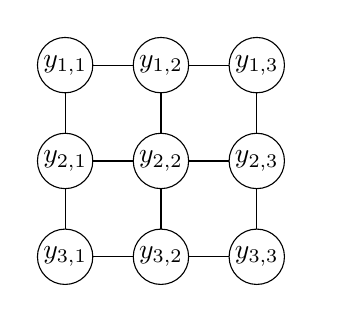
\begin{tikzpicture}
\matrix [row sep=0.5cm, column sep=0.5cm] {
\node(a)[latent]{$y_{1,1}$}; & \node(d)[latent]{$y_{1,2}$}; & \node(g)[latent]{$y_{1,3}$}; & \\
\node(b)[latent]{$y_{2,1}$}; & \node(e)[latent]{$y_{2,2}$}; & \node(h)[latent]{$y_{2,3}$}; & \\
\node(c)[latent]{$y_{3,1}$}; & \node(f)[latent]{$y_{3,2}$}; & \node(i)[latent]{$y_{3,3}$}; & \\
};
\draw(a) -- (b)--(c);
\draw(d) -- (e) --(f);
\draw(g) -- (h) --(i);
\draw(a) -- (d)--(g);
\draw(b) -- (e)--(h);
\draw(c) -- (f)--(i);
\end{tikzpicture}
\end{center}

\noindent In particular consider a conditional Potts model for image denoising.
The input $x$ will consist of a picture with pixels $x_{ij}$, where each
pixel is one of $K$ different colors and has been perturbed by random
noise. Each random variable $y_{ij}$ represents the color we think
each pixel should take after denoising. Unary potentials represent the
prior belief for that pixel based on its observed value. Neighbor
potentials enforce smoothness of the labeling. Specifically,
$\theta(y_{ij}=k) = 10 * \delta(x_{ij}=k)$, and for all neighboring
pixels $n \in \{(i-1, j), (i+1, j), (i, j-1), (i, j+1)\}$,
\[\theta(y_{i,j}, y_n) =
\begin{cases}
  10 & y_{i,j} = y_n \\
  2 & |y_{i,j} - y_n| = 1 \\
  0 & o.w.
\end{cases}
\]



\noindent This is obviously a simplified and discretized view of the true denoising problem,
but it gives us a reasonable place to start. As an example consider the problem with $K=2$
and noise over the image of a spiral.

\begin{center}
  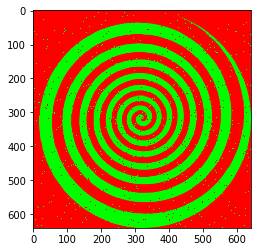
\includegraphics[width=6cm]{spiral}
\end{center}


\noindent [Note: for the example problems we will show k=1 as red, k=2
as green, and k=3 as blue.  We will represent this as the last
dimension of the image in a one-hot encoding, so $x[i,j,0] = 1$ for
red, $x[i,j,1] = 1$ for green, and $x[i,j,2] = 1$ for blue. Here red
is ``close'' to green and green is close to blue, but red is not close
to blue. This is not supposed to be physically true, just part of the problem.]

\newpage

\begin{problem}[Variational Inference for Denoising, 30pts]

\noindent For the problems below we have provided a set of example images in
the form of numpy arrays including a small sample, a flag, a bullseye,
and the large spiral above.

\begin{enumerate}

\item First as a sanity check, consider  the 3x3 image small with $K=2$. Compute using brute-force the
  true posterior marginal probability $p(y_{i,j} | x)$ of any node.

\item Now consider a variational-inference based approach to this
  problem. Using mean-field factorization, with $q(y)$ factored to
each node of the graph, derive local mean field updates.

\begin{center}
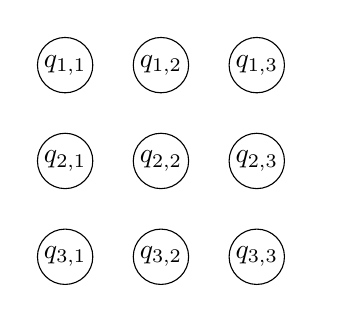
\begin{tikzpicture}
\matrix [row sep=0.5cm, column sep=0.5cm] {
\node(a)[latent]{$q_{1,1}$}; & \node(d)[latent]{$q_{1,2}$}; & \node(g)[latent]{$q_{1,3}$}; & \\
\node(b)[latent]{$q_{2,1}$}; & \node(e)[latent]{$q_{2,2}$}; & \node(h)[latent]{$q_{2,3}$}; & \\
\node(c)[latent]{$q_{3,1}$}; & \node(f)[latent]{$q_{3,2}$}; & \node(i)[latent]{$q_{3,3}$}; & \\
};
\end{tikzpicture}
\end{center}


\item Implement these mean-field updates with a synchronous schedule
  in PyTorch/numpy. (This means that all parameters are updated with
  expectations from the previous time step.). Run for 30 epochs
  starting with $q$ set to a uniform distribution. Graph the results
  on the small images and compare to the brute-force approach. Compare
  the variational values to the exact marginals for the small
  example. Note: running on the spiral example will likely require a
  fast/matrix implementation.

\item Implement Loopy Belief Propagation with a synchronous or
  non-synchronous schedule in PyTorch/Numpy following the algorithm
  given in Murphy (Section 22.2.2). Run for 30 epochs using the
  starting conditions in in Algorithm 22.1. Compare to the mean field
  approach.

\item (Optional)  Write out the Integer Linear Programming formulation for the
  maximum assignment problem. 
  What is the advantage of mean field
  compared to the ILP approach?

\item (Optional) Install the PuLP toolkit in python. Implement the ILP
  formulation for this problem. Compare your solution for the smaller
  images.

\end{enumerate}
\end{problem}
\begin{enumerate}
	\item See code solution. The posterior marginal probability is given by
	
	\begin{verbatim}
	[[[  1.0000e+00   5.7991e-12   9.3612e-14]
		[  1.0000e+00   1.9552e-15   4.2487e-18]
		[  1.0000e+00   5.7991e-12   9.3612e-14]]
		
		[[  1.0000e+00   1.5193e-08   9.3349e-14]
		[  1.0000e+00   6.5694e-12   4.2410e-18]
		[  1.0000e+00   1.5193e-08   9.3349e-14]]
		
		[[  2.5238e-03   9.9748e-01   2.0611e-09]
		[  2.4846e-03   9.9752e-01   7.4111e-13]
		[  2.5238e-03   9.9748e-01   2.0611e-09]]]
	\end{verbatim}
	
	\item We have the target distribution
	\[
	\log p(y\given x) = \sum_{s\sim t} \theta(y_s, y_t) + \sum_{t} \theta_t(y_t) + const
	\]
	Dropping all terms without $y_i$ and taking expectations w.r.t. $y_j: j\neq i$, the update is
	\[
	\log q_i(y_i) = \theta_i(y_i) + \sum_{n\in ngh(i)} \sum_{y_n = 1}^K \theta(y_i, y_n) q_n(y_n) + const
	\]
	
	\item See code solution. See figure ~\ref{1} for results on the images. On the small example, we obtain the following variational values:
	
	\begin{verbatim}
	[[[  1.0000e+00   5.1091e-12   9.3576e-14]
	[  1.0000e+00   1.7139e-15   4.2484e-18]
	[  1.0000e+00   5.1091e-12   9.3576e-14]]
	
	[[  1.0000e+00   1.5219e-08   9.3534e-14]
	[  1.0000e+00   5.1091e-12   4.2484e-18]
	[  1.0000e+00   1.5219e-08   9.3534e-14]]
	
	[[  4.5398e-05   9.9995e-01   2.0611e-09]
	[  1.5252e-08   1.0000e+00   6.9182e-13]
	[  4.5398e-05   9.9995e-01   2.0611e-09]]]
	\end{verbatim}
	The variational values are almost exactly the same as the exact marginals, with the largest difference in value (on the order of $10^{-3}$) occurring at (2, 0) and (2, 1).
	\begin{figure}
		\centering
		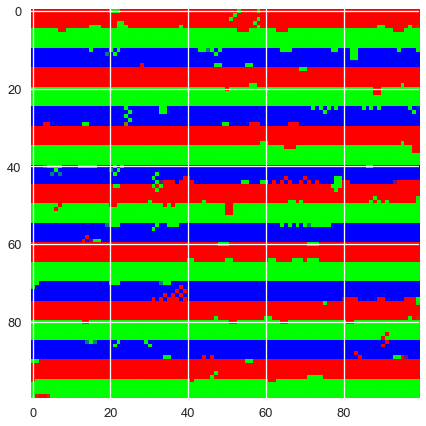
\includegraphics[width=.3\textwidth]{flag_mf}
		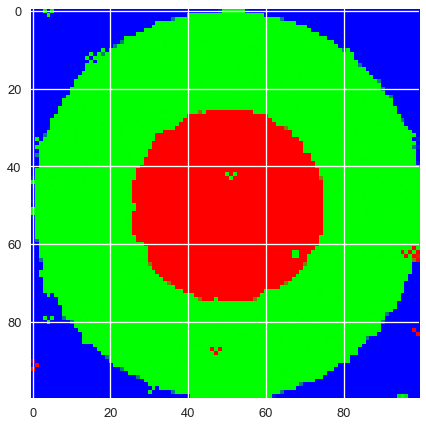
\includegraphics[width=.3\textwidth]{bullseye_mf}
		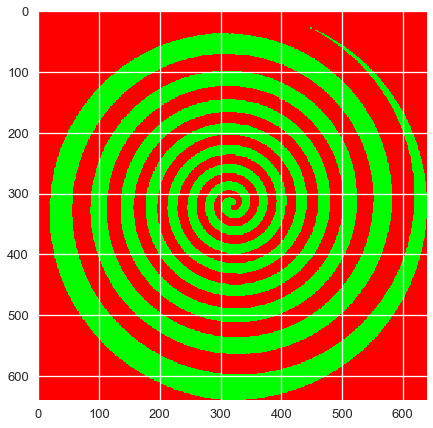
\includegraphics[width=.3\textwidth]{spiral_mf}
		\caption{Denoised images for Mean Field}
		\label{1}
	\end{figure}

	\item See code solution. See figure ~\ref{2} for results on the images. The results for LBP appear to be better than those for MF; region boundaries are much less pixelated and fewer anomalies remain. This makes sense because (1) checkerboard patterns often occur when MF is used without damping and (2)  LBP is generally more accurate than MF since it optimizes over both node and edge potentials, unlike MF, which only optimizes over node potentials.
	\begin{figure}
		\centering
		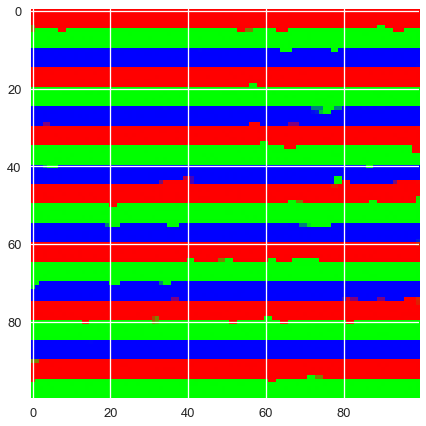
\includegraphics[width=.3\textwidth]{flag_lbp}
		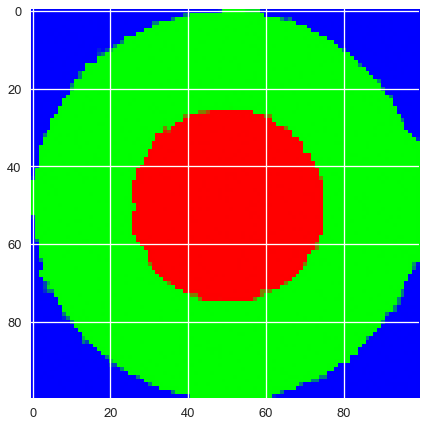
\includegraphics[width=.3\textwidth]{bullseye_lbp}
		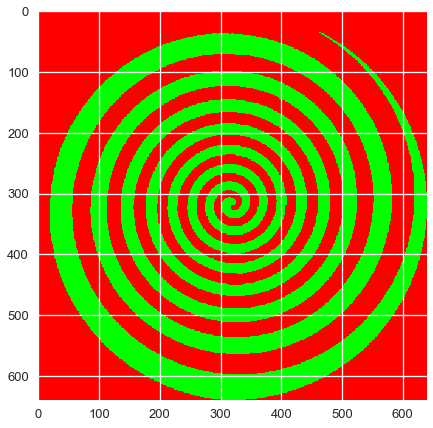
\includegraphics[width=.3\textwidth]{spiral_lbp}
		\caption{Denoised images for LBP}
		\label{2}
	\end{figure}

	\item We have the Integer LP:
	\begin{align*}
	\max_{y} &\ \ \sum_{s\sim t} \theta(y_s, y_t) + \sum_{t} \theta_t(y_t) \\
	\text{subject to} &\ \ y_t\in\{1,\dots,K\} \ \forall t
	\end{align*}
	Unfortunately, the marginal polytope of $y$ in general has a number of facets that is exponential in the number of nodes, making the ILP difficult to solve without relaxations.
	
\end{enumerate}


\newpage
\section*{Modeling users and jokes with a Bayesian latent bilinear model}

The next two questions will develop Bayesian inference methods for the simplest version of the latent bilinear model you used to model jokes ratings in HW3. The data set we'll use is the same as in HW3, a modified and preprocessed variant of the Jester data set. However, to make things easier (and to make being Bayesian more worthwhile) {\bf we'll only use subsampling to 10\% of the training data}.  The other ratings will form your test set.

\subsection*{The model}

The model is the same as in HW3, but with Gaussian priors on the latent parameter matrices $U$ and $V$. Let~${r_{i,j}\in\{1,2,3,4,5\}}$ be the rating of user $i$ on joke $j$.  A latent linear model introduces a vector ${u_i\in\R^K}$ for each user and a vector~${v_j\in\R^K}$ for each joke.  Then, each rating is modeled as a noisy version of the appropriate inner product. Specifically,
\[
r_{i,j} \sim \mathcal{N}(u_i^T v_j, \sigma_\epsilon^2).
\]
Fix $\sigma_\epsilon^2$ to be 1.0, and start with $K = 2$. We put independent Gaussian priors on each element of $U$ and $V$:
\[U_{i,k} \sim \mathcal{N}(0, \sigma_U^2=5)\]
\[V_{j,k} \sim \mathcal{N}(0, \sigma_V^2=5)\]

\begin{problem}[Stochastic Variational Inference, 30pts]

Recall that variational inference optimizes a lower bound on the log marginal likelihood (integrating out parameters $\theta$), like so:
\begin{align}
\log p(x) & = \log \int p(x, \theta) d\theta = \log \int p(x|\theta) p(\theta) d\theta \\
& = \log \int \frac{q_\lambda(\theta)}{q_\lambda(\theta)} p(x|\theta) p(\theta) d\theta
  = \log \mathbb{E}_{q_\lambda} \frac{1}{q(\theta)} p(x|\theta) p(\theta) d\theta \\
& \geq \mathbb{E}_{q_\lambda} \log \left[ \frac{1}{q_\lambda(\theta)} p(x|\theta) p(\theta) \right]
 = \underbrace{-\mathbb{E}_{q_\lambda} \log q_\lambda(\theta)}_{\textnormal{entropy}}  + \underbrace{\mathbb{E}_{q_\lambda} \log p(\theta)}_{\textnormal{prior}} + \underbrace{\mathbb{E}_{q_\lambda} \log p(x|\theta)}_{\textnormal{likelihood}}
= \mathcal{L}(\lambda)
\end{align}
%
In this case, $\theta = U,V$ and $x = R$:
%
\begin{align}
\mathcal{L}(\lambda) = -\mathbb{E}_{q_\lambda} \log q_\lambda(U, V) + \mathbb{E}_{q_\lambda} \log p(U, V) + \sum_{n=1}^N \mathbb{E}_{q_\lambda} \log p(r_n | U, V)
\end{align}
%

\noindent This is a general formula that works for many different priors, likelihoods and variational approximations. 
Here we will keep things simple and choose $q(U,V)$ to be a Gaussian factorized over every single entry of each matrix for $U$ and $V$, e.g. the same form as the prior.
Thus our variational parameters will consist of a mean and variance for each entry in U and V: $\lambda^{(\mu U)}_{ik}$, $\lambda^{(\sigma^2 U)}_{ik}$, $\lambda^{(\mu V)}_{jk}$, 
and $\lambda^{(\sigma^2 V)}_{jk}$.

\begin{enumerate}

\item Derive the expression for the $KL$ divergence between two univariate Gaussians.

\item Exploiting the conditional independence of the model, we can write the variational objective (which we want to maximize) as:
\[ {\cal L}(\lambda) = -KL(q_\lambda(U)\ ||\  p(U) ) - KL(q_\lambda(V)\ ||\ p(V)) + \sum_{n=1}^N \mathbb{E}_{q_\lambda} \log p(r_n | U, V)\]

Simplify the first two terms of this model to get a closed form expression.


\item The third term is the likelihood of the data under an expectation wrt the variational parameters.
  Assume that we approximate this term using a single sample of rows $\tilde{u}_{i}$  and $\tilde{v}_{j}$
  for each rating $r_{i,j}$. Write out the full objective with this approximation for the last term.

\item  Unfortunately this is difficult to optimize, since the sampled variables 
depend on the variational parameters $\lambda$. An alternative method, known as 
\textit{reparameterization}, replaces expectation of the form 
$\mathbb{E}_{X \sim \mathcal{N}(\mu, \sigma^2)}[f(X)]$, in terms of 
$\mathbb{E}_{Z \sim \mathcal{N}(0, 1)}[f(Z \sigma + \mu)]$. Rewrite the 
objective in this form using sampled dummy variables $\tilde{z}$ 
(and no $\tilde{u}_{i}$  or $\tilde{v}_{j})$.

\item Using PyTorch, set up this model using \texttt{nn.Embedding} for the variational parameters. For numerical stability, store the log of the variance in
  the embedding table, and also initialize this table with very low values, e.g. \texttt{logvar.weight.data = -10}. 
  For $K = 2$, optimize the variational parameters for 10 epochs over the sampled data.  Use Adam with learning rate 0.001.

Plot the training and test-set log-likelihood as a function of the number of epochs, as well as the marginal likelihood lower bound.
That is to say: at the end of each epoch, evaluate the log of the average predictive probability of all ratings in the training and test sets using 100 samples from q(U,V).
The lower bound is the sum of entropy, prior and likelihood terms, while the training-set and test-set likelihoods only use the likelihood term.

\item Fit your variational model for $K = 1$ to $K = 10$, and plot the training-set log-likelihood, test-set log-likelihood, and lower bound for each value of $K$.
How do the shapes of these curves differ?



\end{enumerate}
\end{problem}
\begin{enumerate}
	\item Let $p(x) = \N(x\given \mu_1, \sigma_1^2)$ and $q(x) = \N(x\given \mu_2, \sigma_2^2)$. We have the following:
	\begin{align*}
	KL(p||q) 
	&= \int p(x) \log p(x) dx - \int p(x) \log q(x) dx \\
	&= - \frac{1}{2} (1 + \log 2 \pi \sigma_1^2) + \frac{1}{2} \log (2 \pi \sigma_2^2) + \frac{\sigma_1^2 + (\mu_1 - \mu_2)^2}{2 \sigma_2^2} \\
	&= \log \frac{\sigma_2}{\sigma_1} + \frac{\sigma_1^2 + (\mu_1 - \mu_2)^2}{2 \sigma_2^2} - \frac{1}{2}
	\end{align*}
	
	\item We use the priors described in the problem specs. Noting that the KL-divergence of products decomposes into the sums of KL-divergences of its parts, we can write
	\begin{align*}
	& KL(q_\lambda(U)\ ||\  p(U) ) + KL(q_\lambda(V)\ ||\ p(V)) \\
	=& \sum_{ik} KL(q_\lambda(U_{ik})\ ||\  p(U_{ik})) + \sum_{jk} KL(q_\lambda(V_{jk})\ ||\  p(V_{jk})) \\
	=& 
	\left[\sum_{ik} \log \frac{\sigma_{U}}{\lambda^{(\sigma U)}_{ik}} + \frac{(\lambda^{(\sigma U)}_{ik})^2 + (\lambda^{(\mu U)}_{ik})^2}{2 \sigma_{U}^2} - \frac{1}{2}\right]
	+ \left[\sum_{jk} \log \frac{\sigma_{V}}{\lambda^{(\sigma V)}_{jk}} + \frac{(\lambda^{(\sigma V)}_{jk})^2 + (\lambda^{(\mu V)}_{jk})^2}{2 \sigma_{V}^2} - \frac{1}{2}\right]
	\\
	=& 
	\left[\sum_{ik} \log \frac{\sigma_{U}}{\lambda^{(\sigma U)}_{ik}} + \frac{(\lambda^{(\sigma U)}_{ik})^2 + (\lambda^{(\mu U)}_{ik})^2}{2 \sigma_{U}^2}\right]
	+ \left[\sum_{jk} \log \frac{\sigma_{V}}{\lambda^{(\sigma V)}_{jk}} + \frac{(\lambda^{(\sigma V)}_{jk})^2 + (\lambda^{(\mu V)}_{jk})^2}{2 \sigma_{V}^2}\right] + const
	\end{align*}
	
	\item We approximate the last term by:
	\[
	\mathbb{E}_{q_\lambda} \log p(r_n\given U, V) 
	\approx \log \N(r_n\given \tilde{u_i}^\top \tilde{v_j}, \sigma_\epsilon^2),
	\]
	where $\tilde{u_{ik}}$ and $\tilde{v_{jk}}$ are sampled so that each $\tilde{u_{ik}} \sim \N(\lambda^{(\mu U)}_{ik}, \lambda^{(\sigma^2 U)}_{ik})$ and each $\tilde{v_{jk}} \sim \N(\lambda^{(\mu V)}_{jk}, \lambda^{(\sigma^2 V)}_{jk})$. 
	
	Our objective is now
	\begin{align*}
	{\cal L}(\lambda) =&
	-\left[\sum_{ik} \log \frac{\sigma_{U}}{\lambda^{(\sigma U)}_{ik}} + \frac{(\lambda^{(\sigma U)}_{ik})^2 + (\lambda^{(\mu U)}_{ik})^2}{2 \sigma_{U}^2}\right]
	- \left[\sum_{jk} \log \frac{\sigma_{V}}{\lambda^{(\sigma V)}_{jk}} + \frac{(\lambda^{(\sigma V)}_{jk})^2 + (\lambda^{(\mu V)}_{jk})^2}{2 \sigma_{V}^2}\right] \\
	&- \sum_{n=1}^N \frac{(r_n - \tilde{u_i}^\top \tilde{v_j})^2}{2\sigma_\epsilon^2}
	+ const
	\end{align*}
	
	\item We rewrite the last term as:
	\[
	\mathbb{E}_{q_\lambda} \log p(r_n\given U, V) 
	\approx 
	\log \N(r_n\given (\tilde{z}_U \odot\lambda^{(\sigma U)}_i + \lambda^{(\mu U)}_i)^\top (\tilde{z}_V \odot\lambda^{(\sigma V)}_j + \lambda^{(\mu V)}_j), \sigma_\epsilon^2),
	\]
	where $\tilde{z}_U$ and $\tilde{z}_V$ are sampled from $\N(0, I_K)$. 
	
	Our objective is now
	\begin{align*}
	{\cal L}(\lambda) =&
	-\left[\sum_{ik} \log \frac{\sigma_{U}}{\lambda^{(\sigma U)}_{ik}} + \frac{(\lambda^{(\sigma U)}_{ik})^2 + (\lambda^{(\mu U)}_{ik})^2}{2 \sigma_{U}^2}\right]
	- \left[\sum_{jk} \log \frac{\sigma_{V}}{\lambda^{(\sigma V)}_{jk}} + \frac{(\lambda^{(\sigma V)}_{jk})^2 + (\lambda^{(\mu V)}_{jk})^2}{2 \sigma_{V}^2}\right] \\
	&- \sum_{n=1}^N \frac{\left(r_n - (\tilde{z}_U \odot\lambda^{(\sigma U)}_i + \lambda^{(\mu U)}_i)^\top (\tilde{z}_V \odot\lambda^{(\sigma V)}_j + \lambda^{(\mu V)}_j)\right)^2}{2\sigma_\epsilon^2}
	+ const
	\end{align*}
	
	\item See code solution. See figure ~\ref{k2} for graphs of the results for learning rate 0.04. Note that all values are up to a constant additive factor.
	\begin{figure}
		\centering
		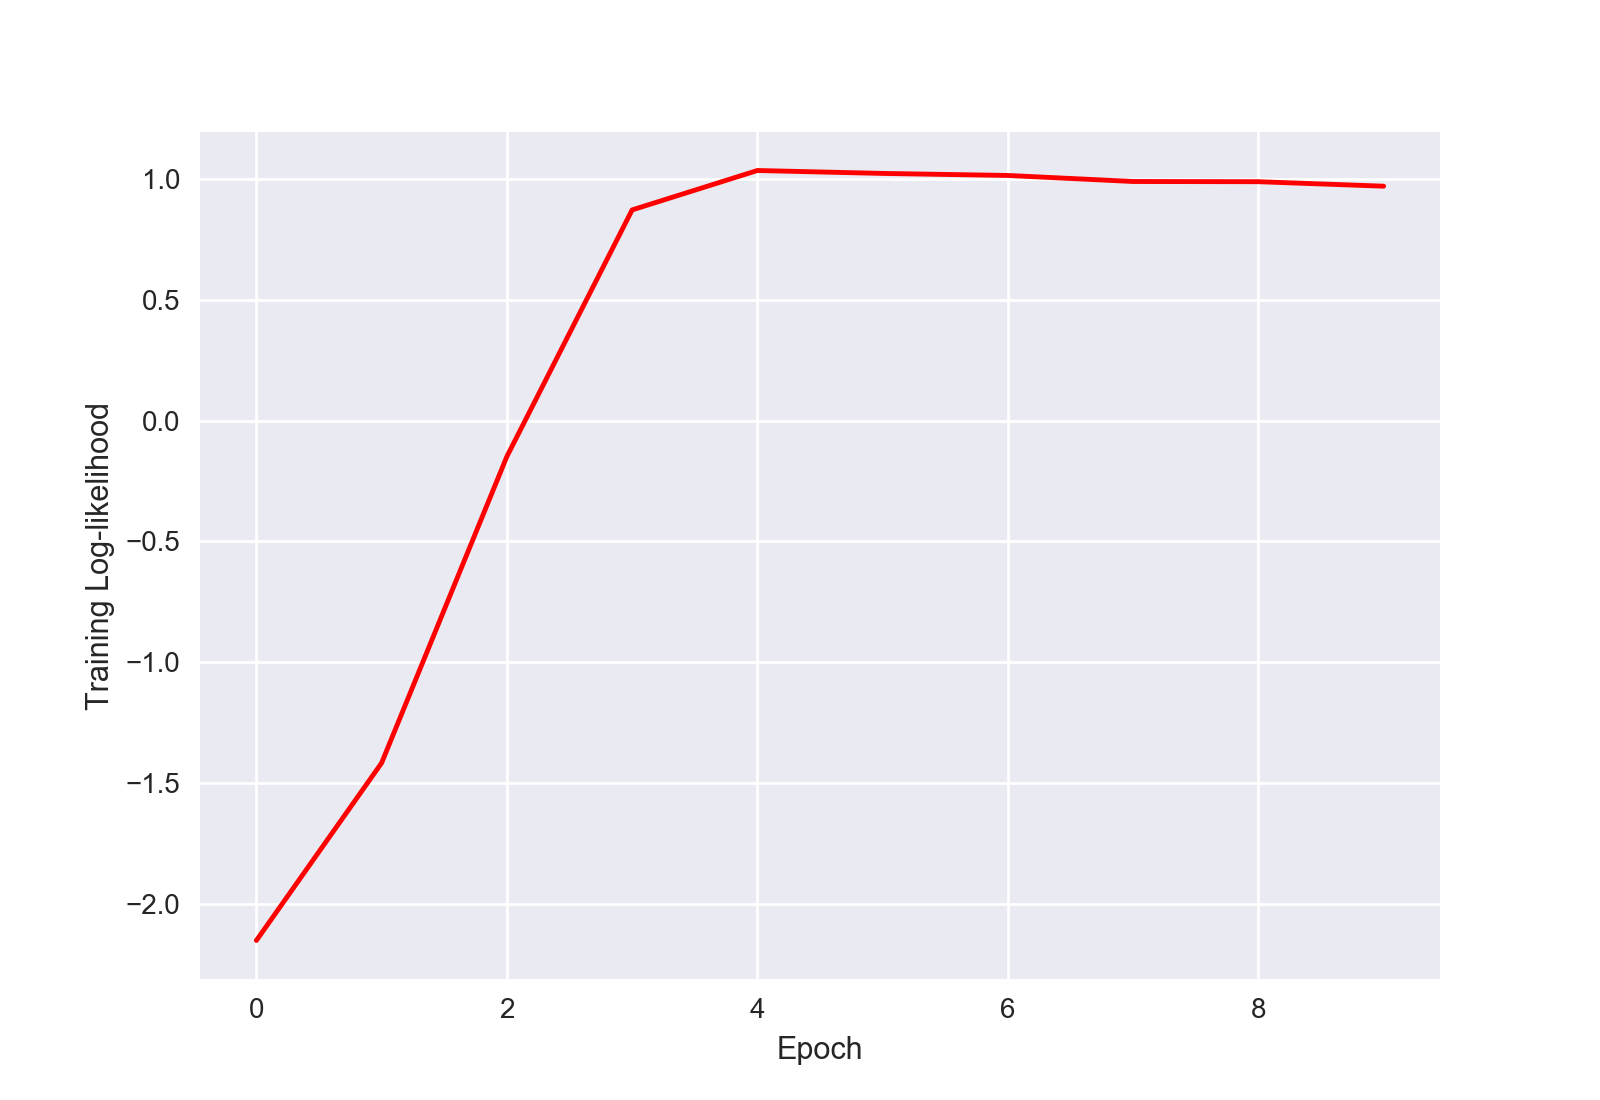
\includegraphics[width=.3\textwidth]{2-1}
		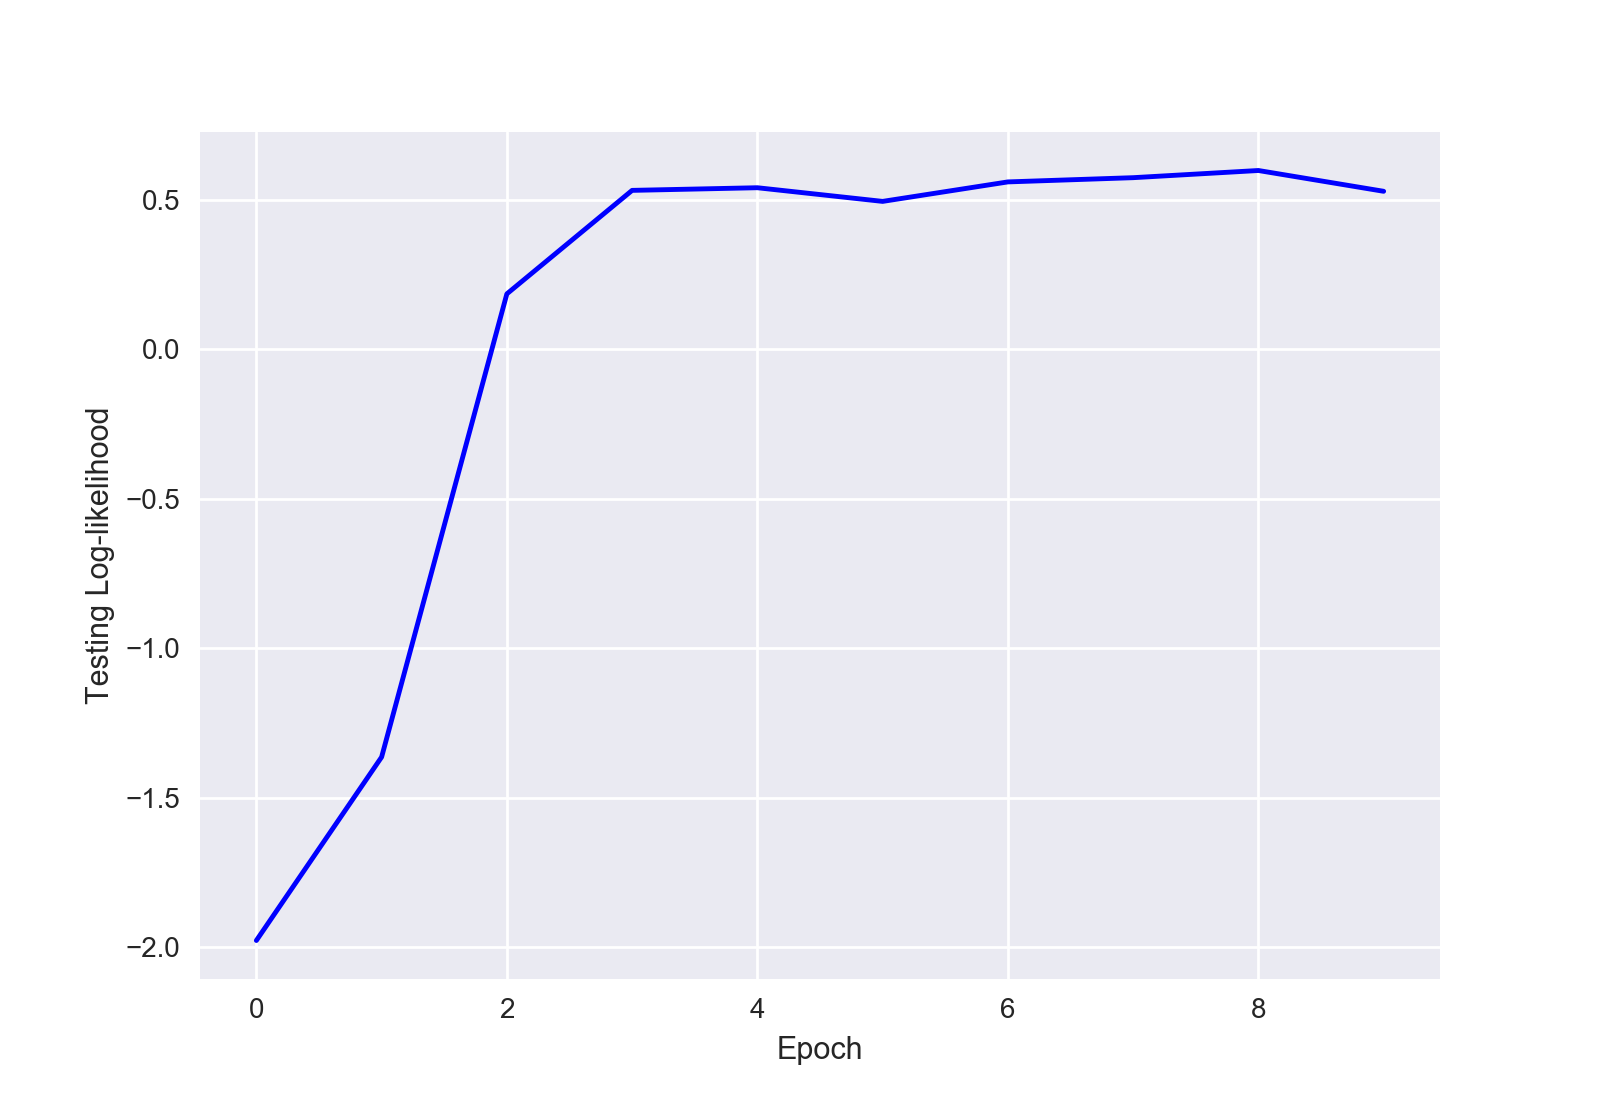
\includegraphics[width=.3\textwidth]{2-2}
		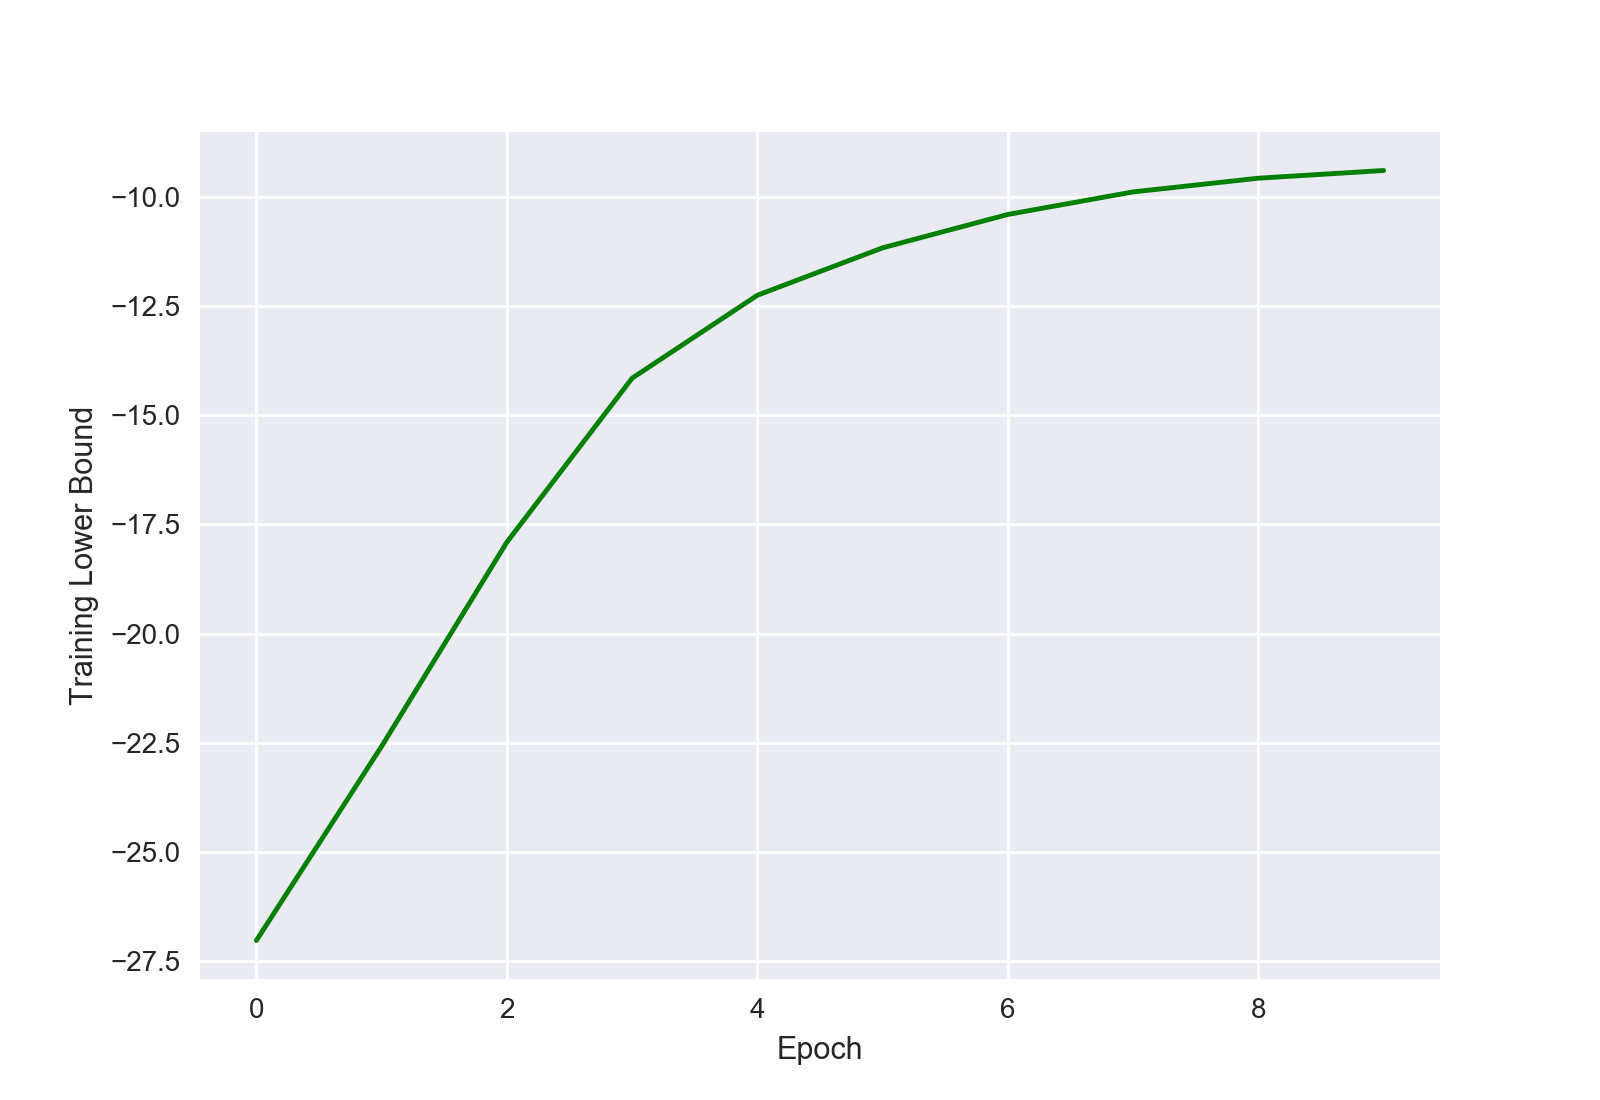
\includegraphics[width=.3\textwidth]{2-3}
		\caption{$K = 2$. Training log-likelihood, testing log-likelihood, and training lower bound for 10 epochs.}
		\label{k2}
	\end{figure}

	\item See code solution. Inspecting the graphs in ~\ref{4},  we can see that the log-likelihood curves plateau after around 4 epochs, indicating convergence. All curves are roughly increasing in epochs. Note that while training log-likelihood curves are roughly comparable across $K$'s, higher $K$ values achieve worse performance on the testing set, which makes sense since there are more parameters to infer and we may be overfitting. Also, as $K$ increases, the lower bound decreases because the penalty on the weights imposed by the prior increases.
	
	\begin{figure}
		\centering
		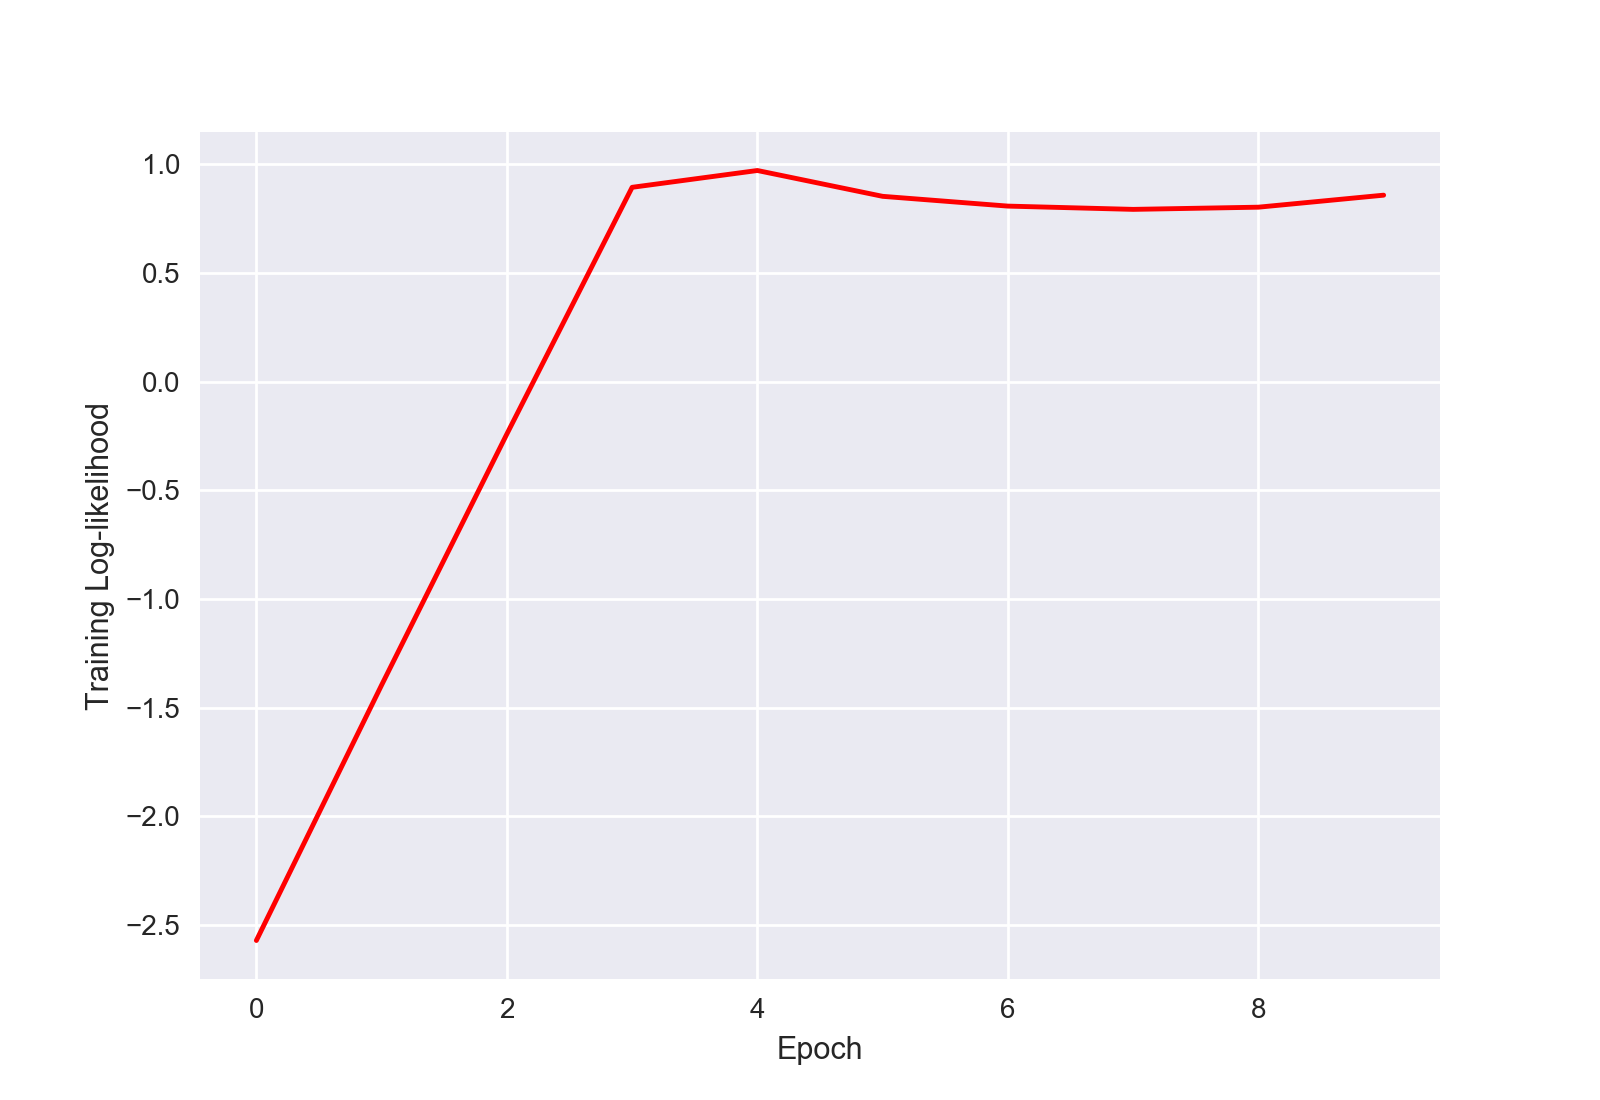
\includegraphics[width=.3\textwidth]{4-1}
		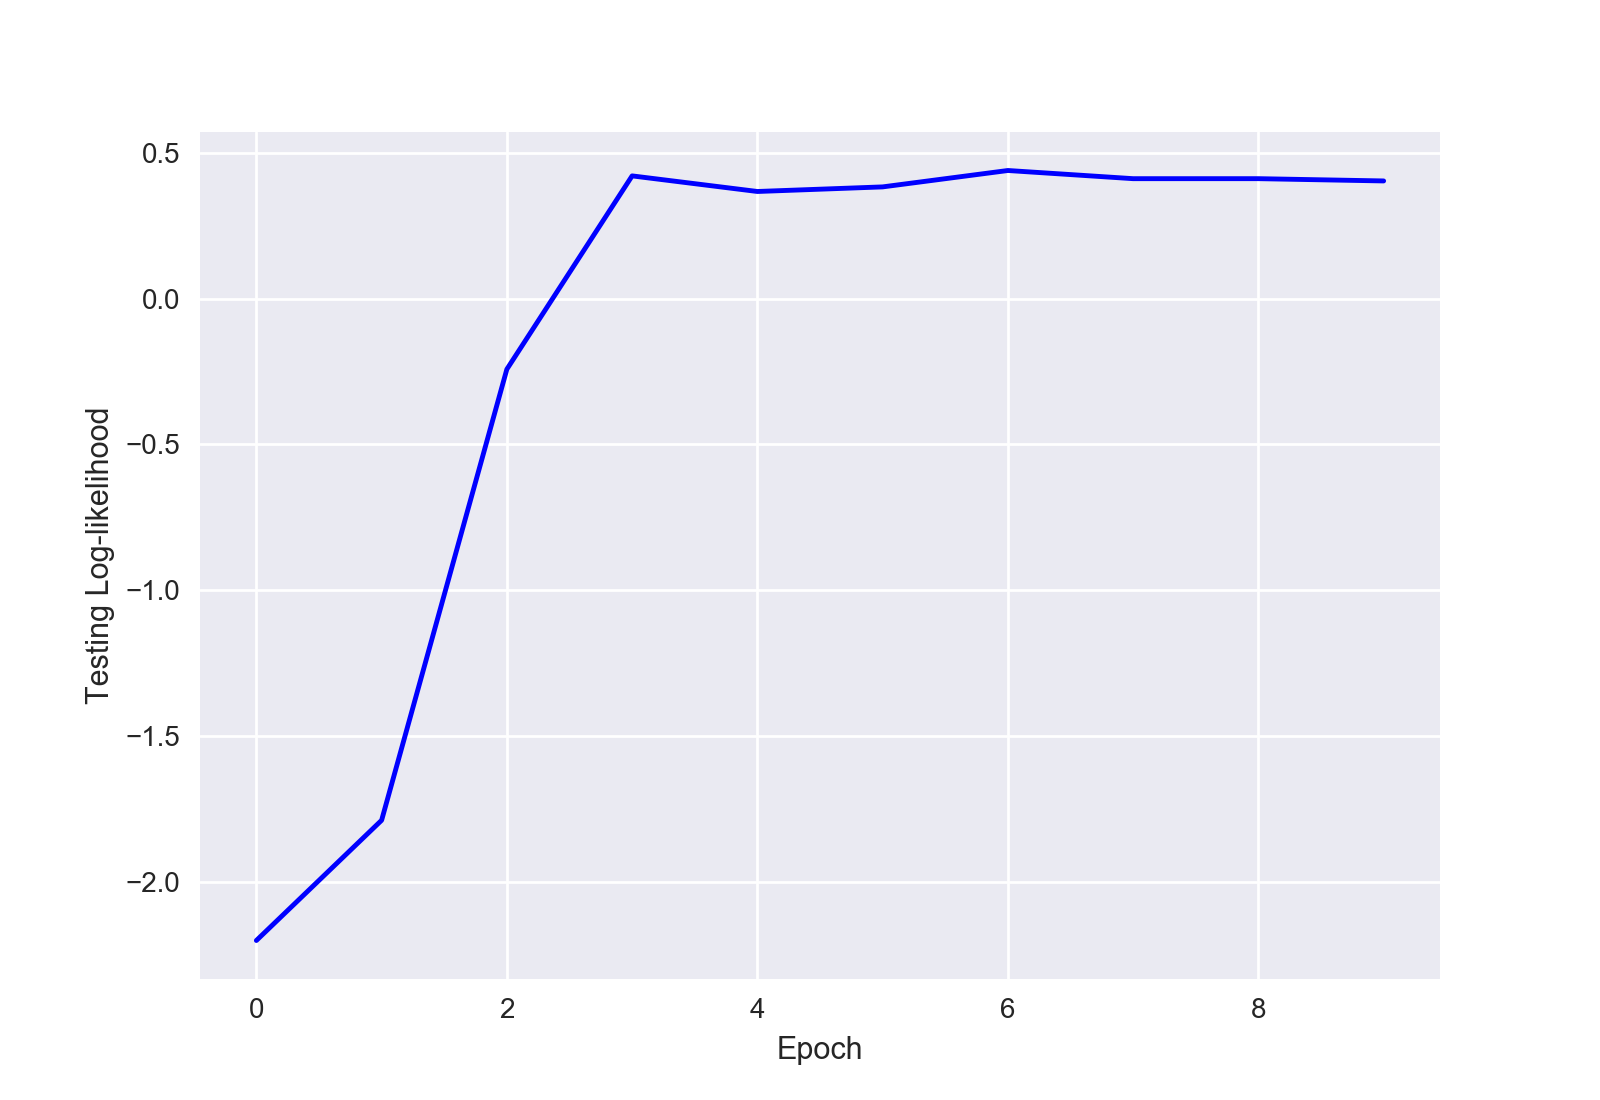
\includegraphics[width=.3\textwidth]{4-2}
		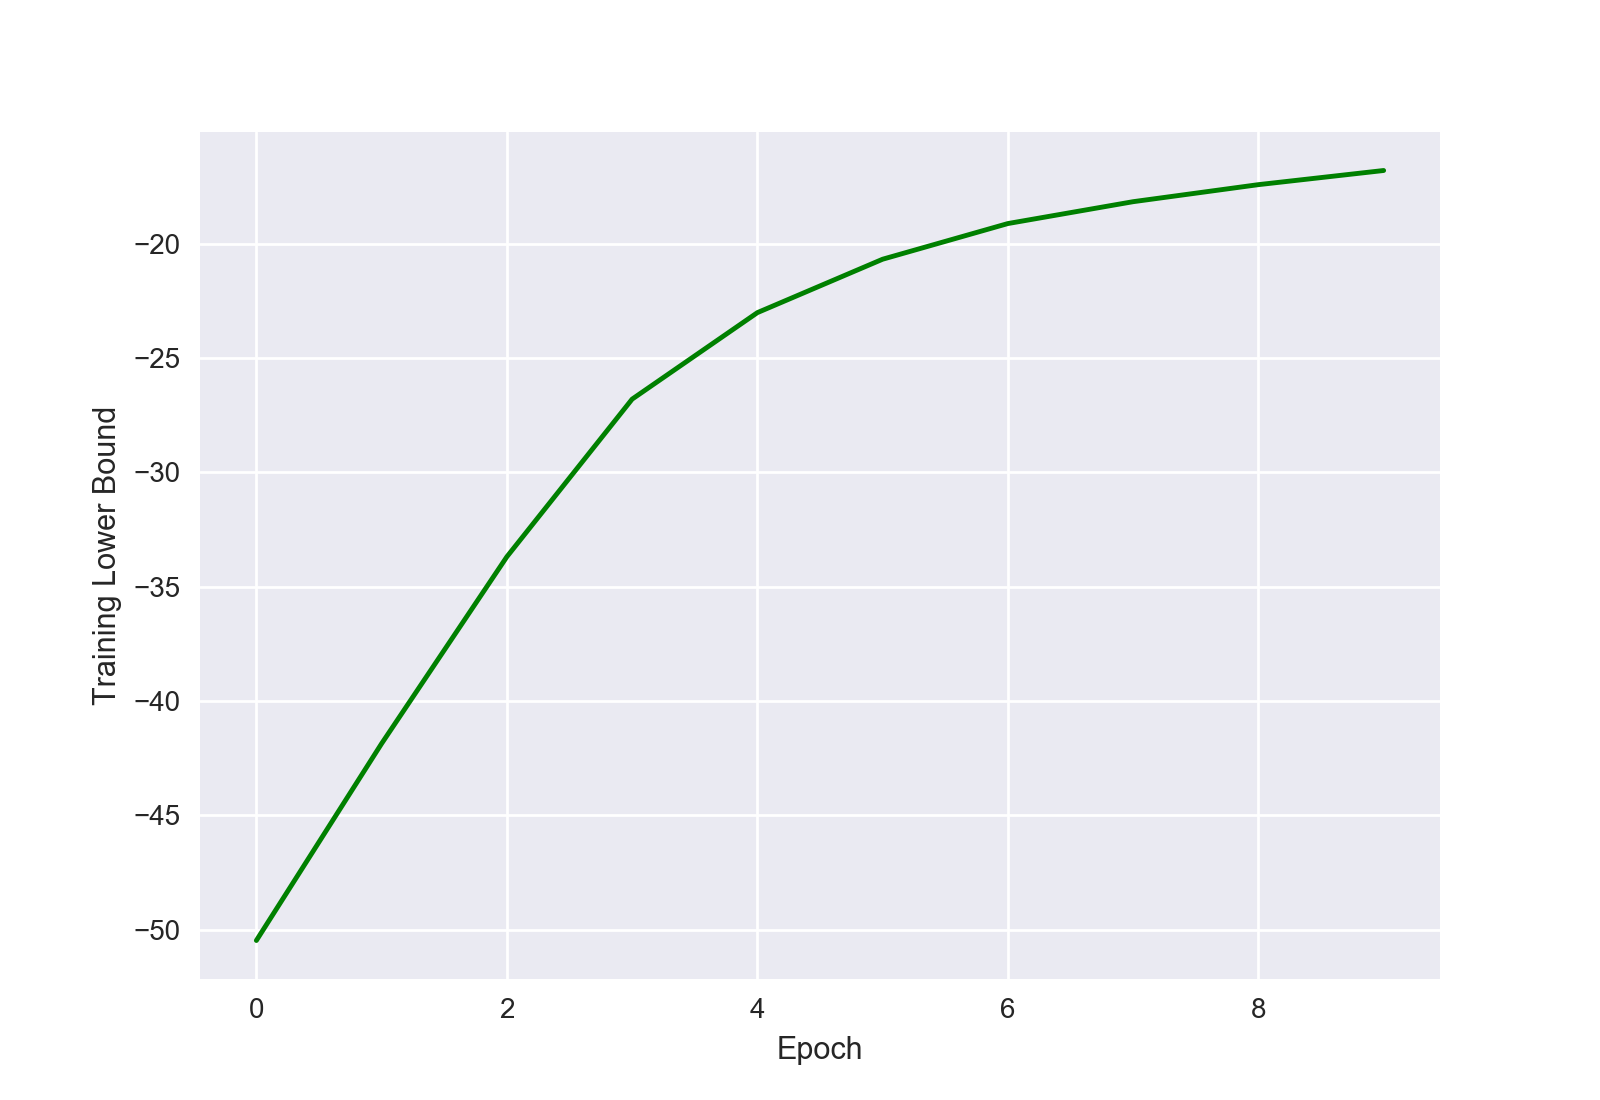
\includegraphics[width=.3\textwidth]{4-3}
		\caption{$K = 4$. Training log-likelihood, testing log-likelihood, and training lower bound for 10 epochs.}
		\label{3}
	\end{figure}
	
	\begin{figure}
	\centering
	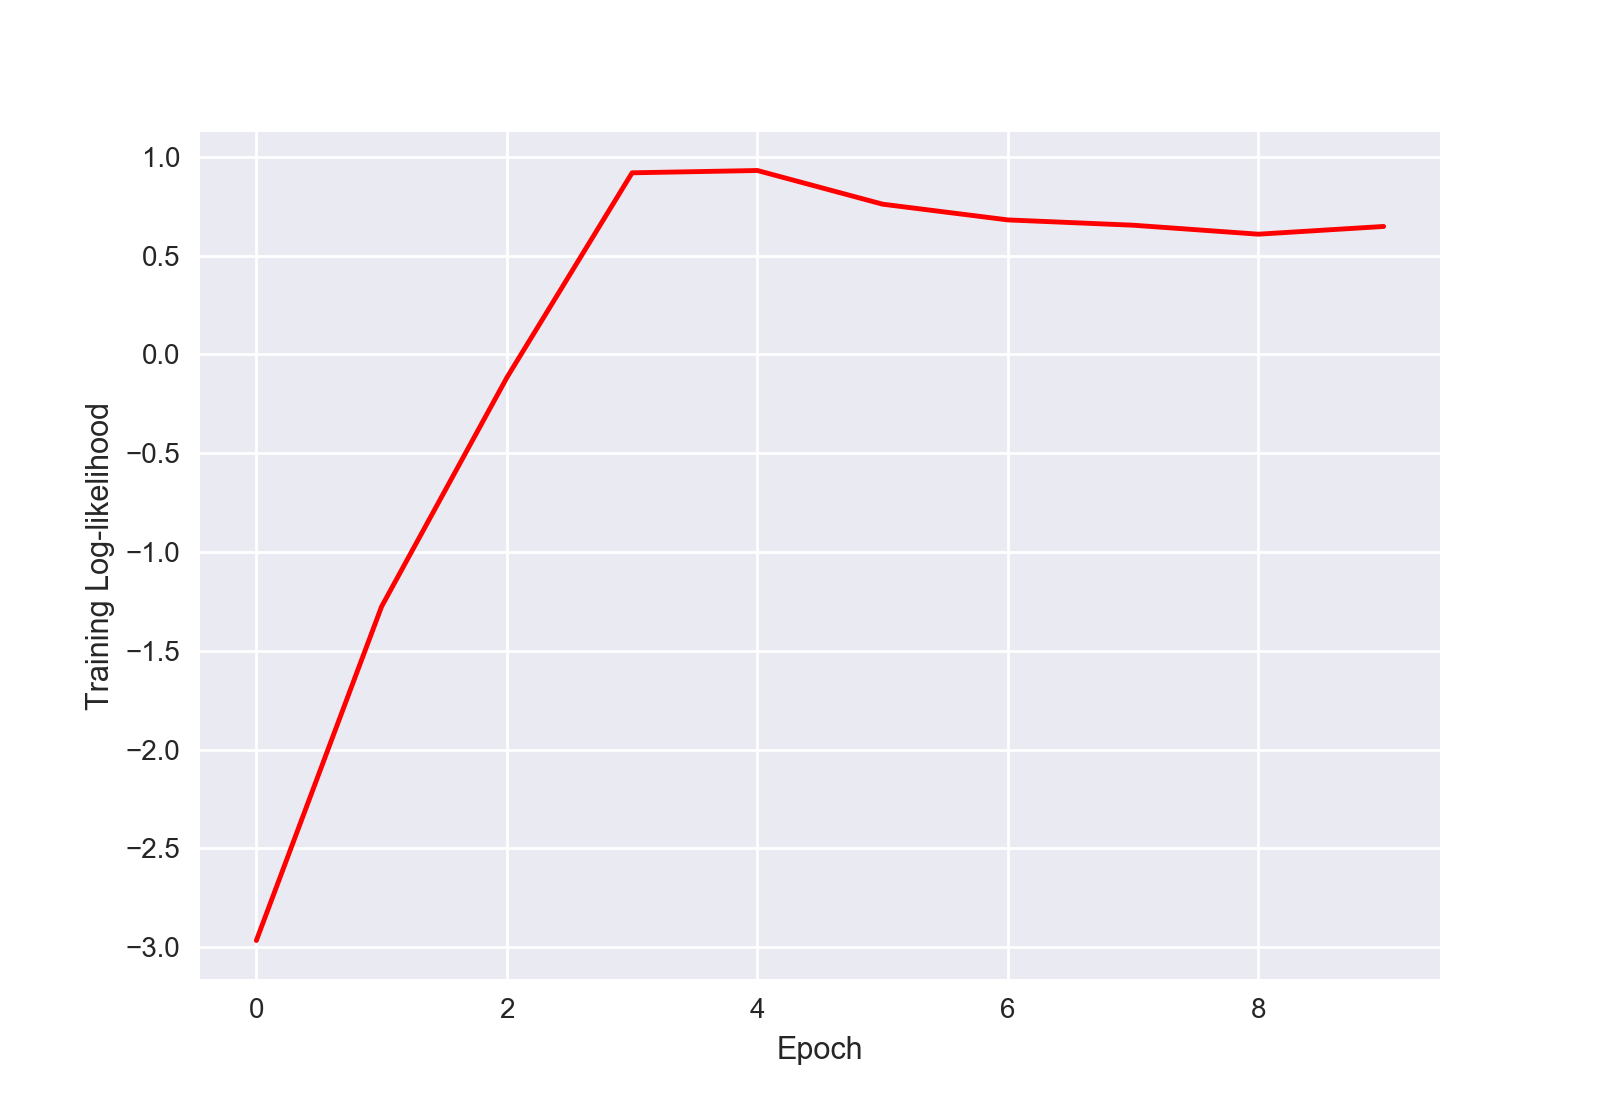
\includegraphics[width=.3\textwidth]{6-1}
	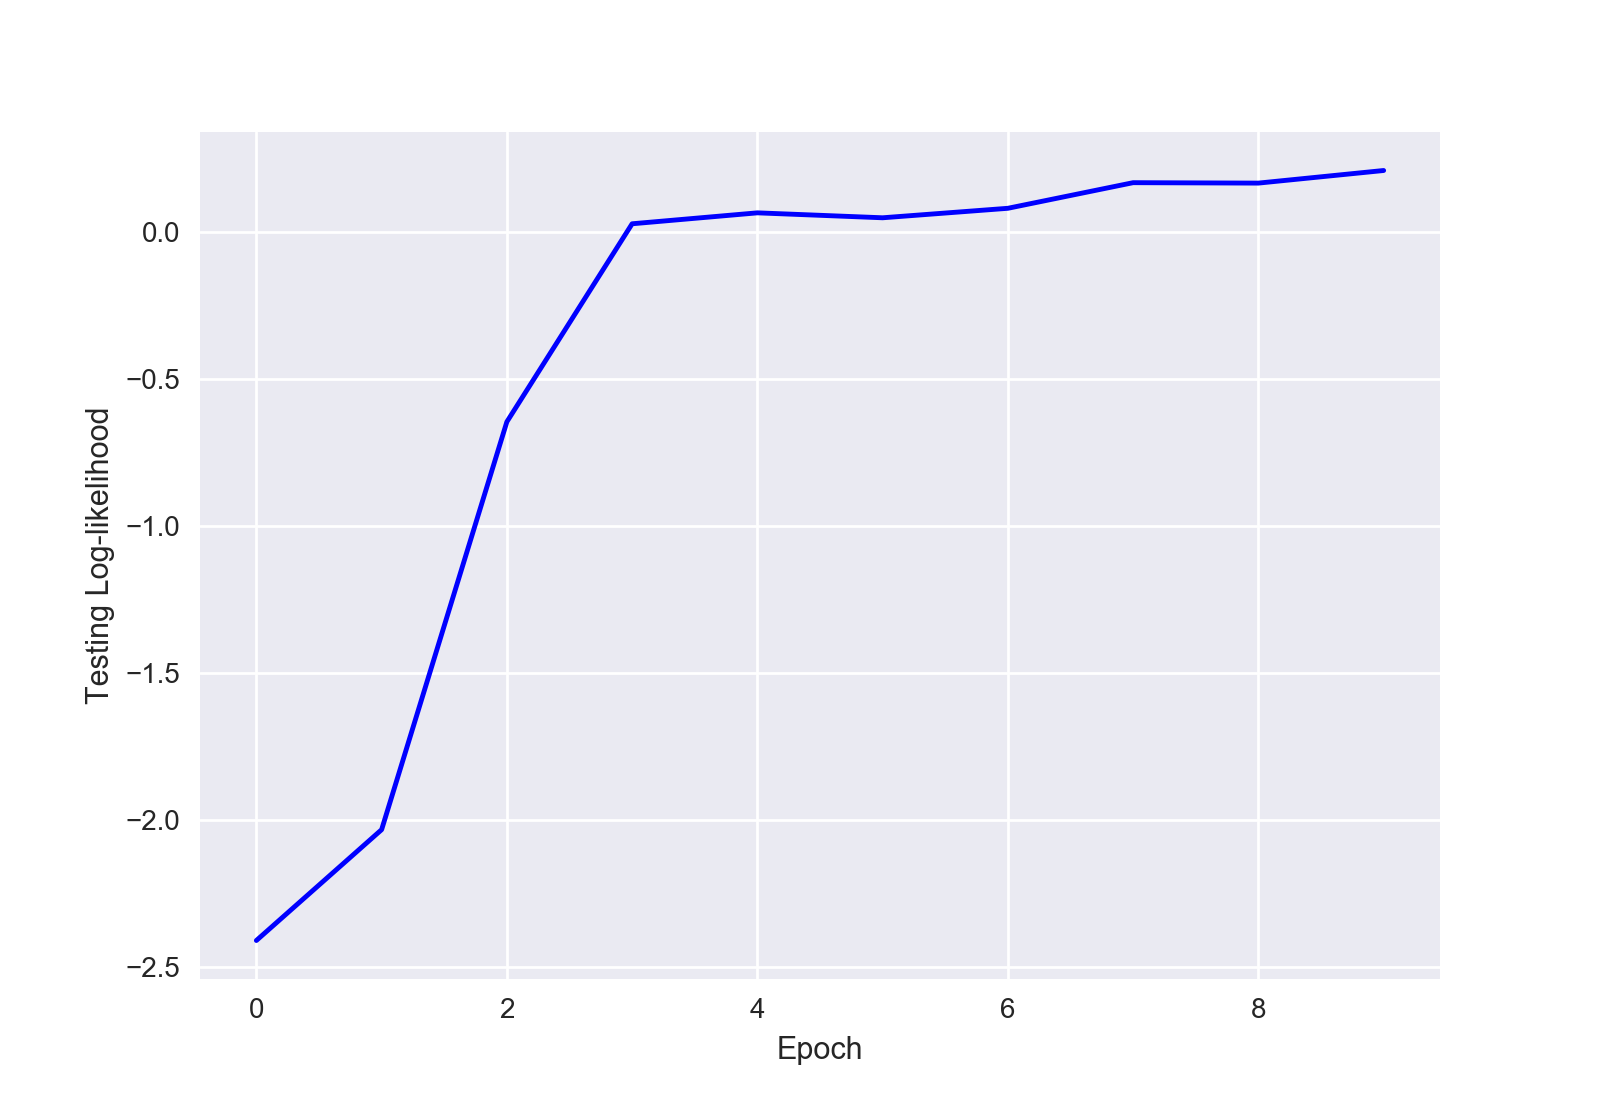
\includegraphics[width=.3\textwidth]{6-2}
	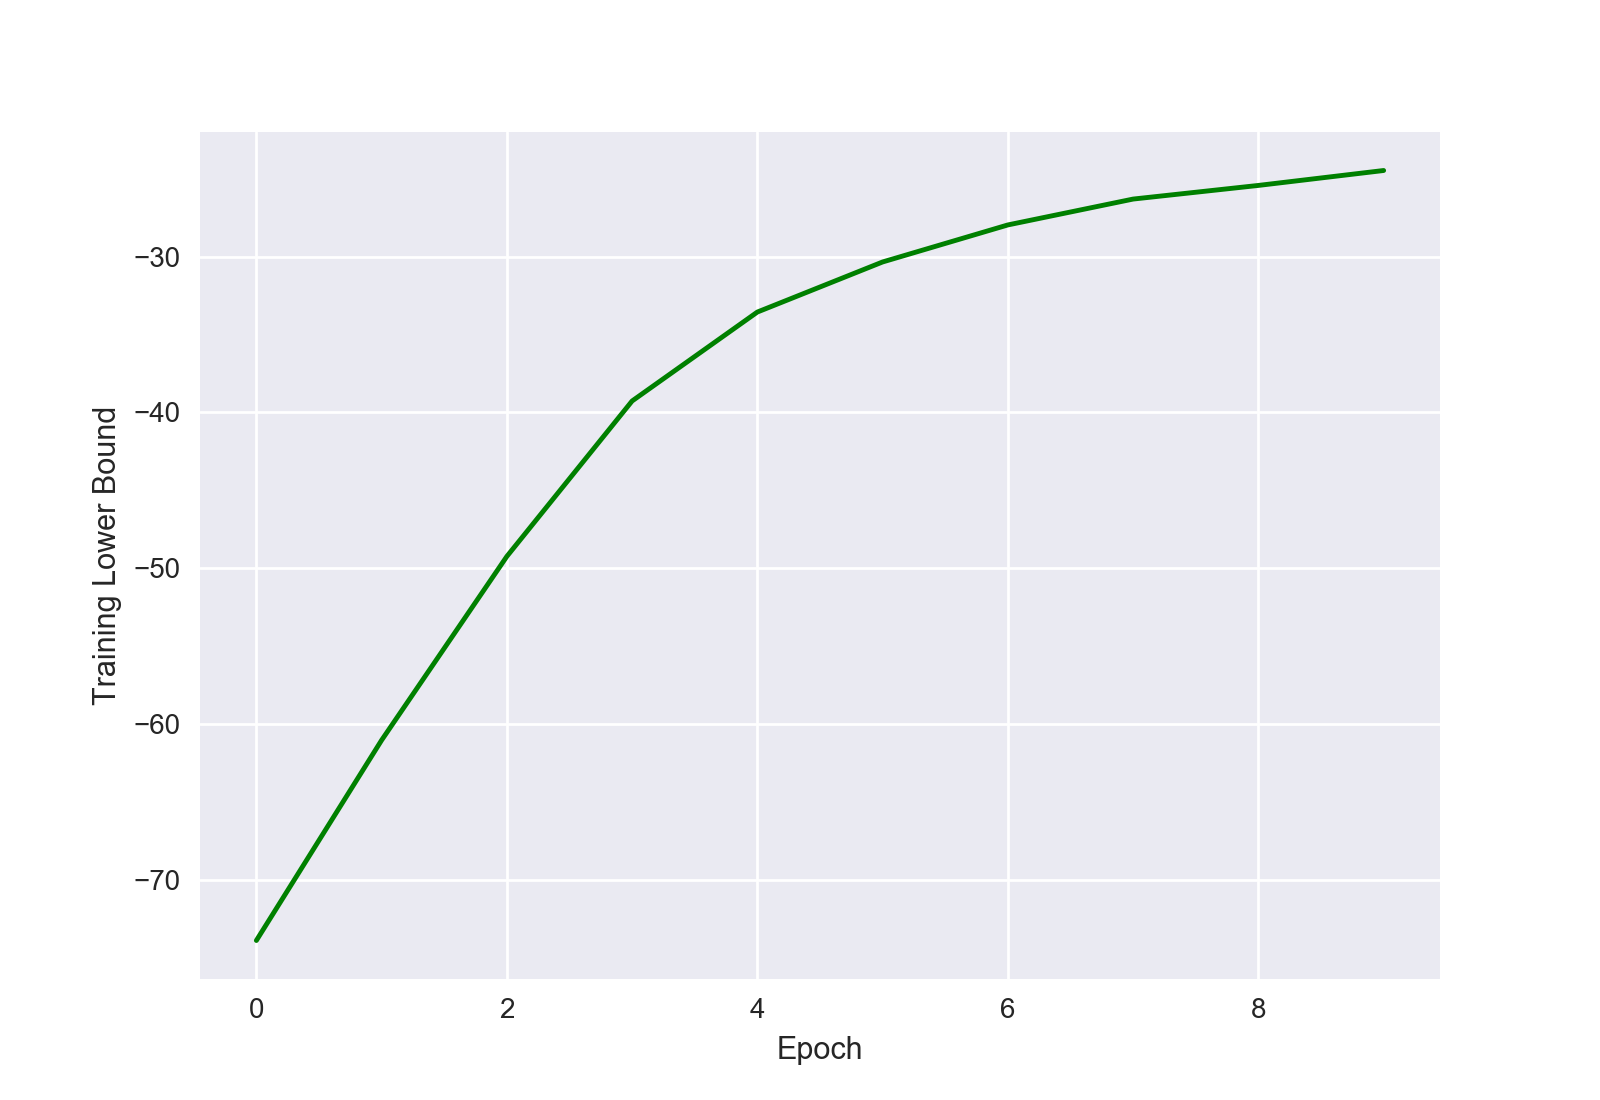
\includegraphics[width=.3\textwidth]{6-3}
	\caption{$K = 6$. Training log-likelihood, testing log-likelihood, and training lower bound for 10 epochs.}
	\label{4}
	\end{figure}

	\begin{figure}
	\centering
	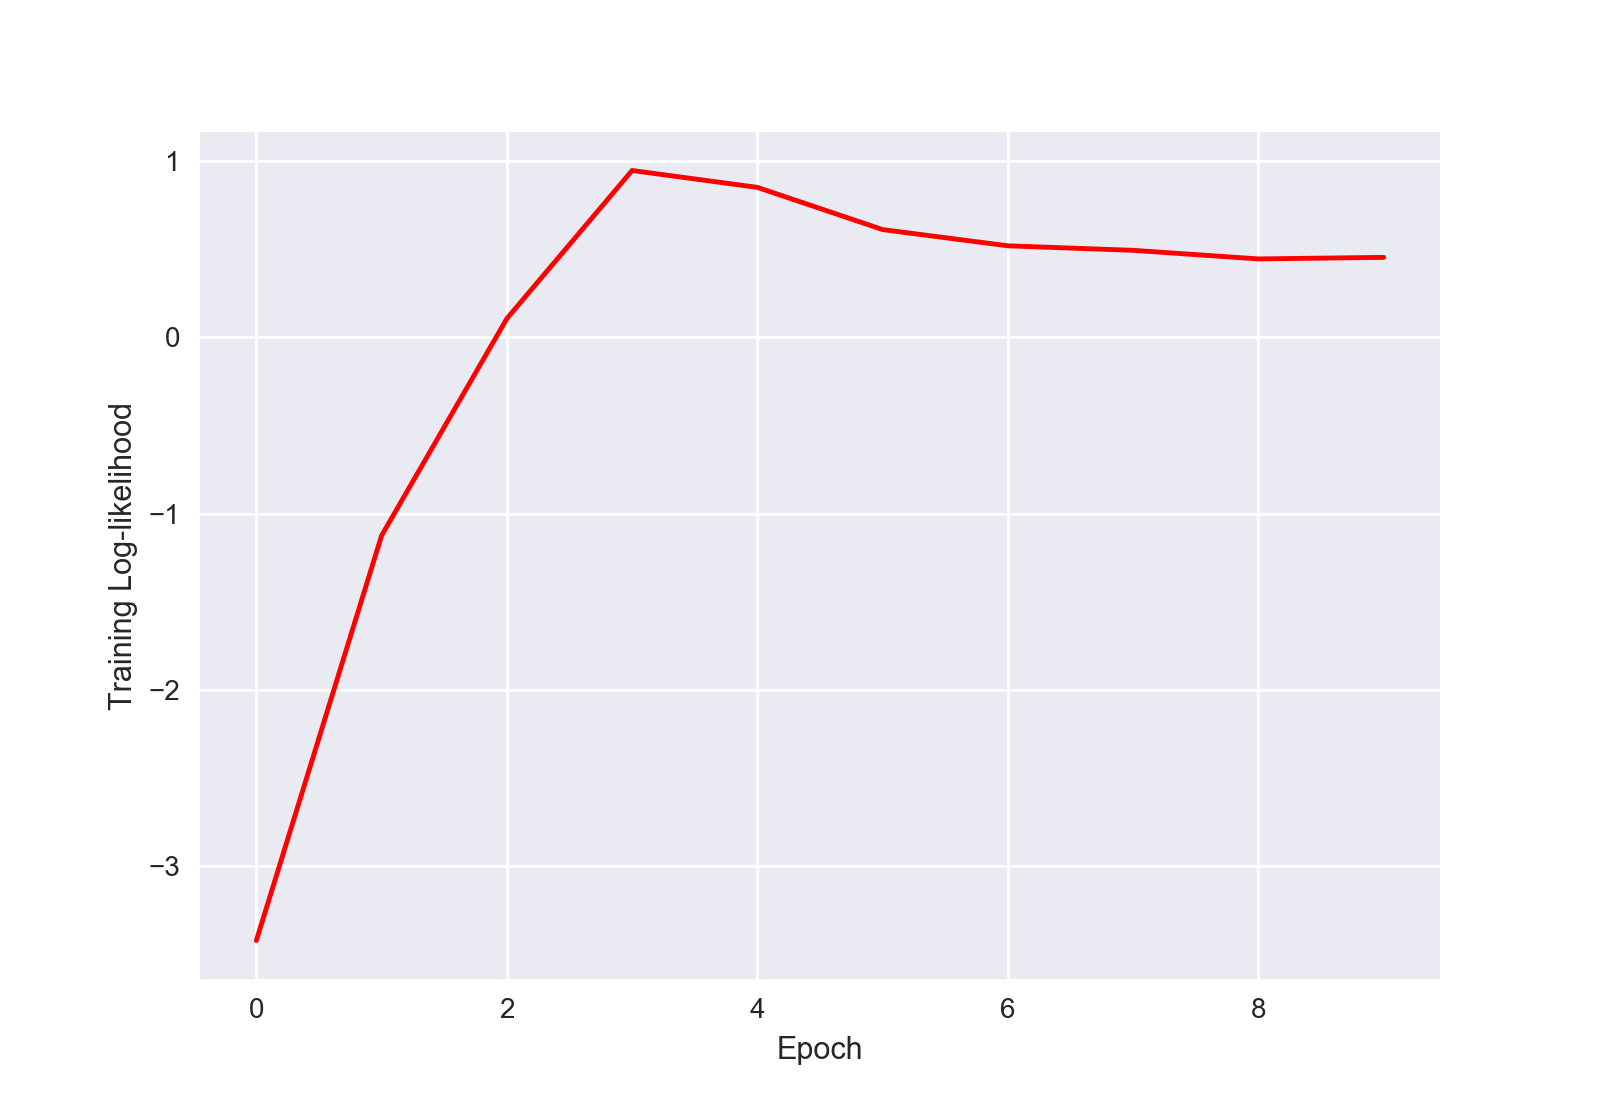
\includegraphics[width=.3\textwidth]{8-1}
	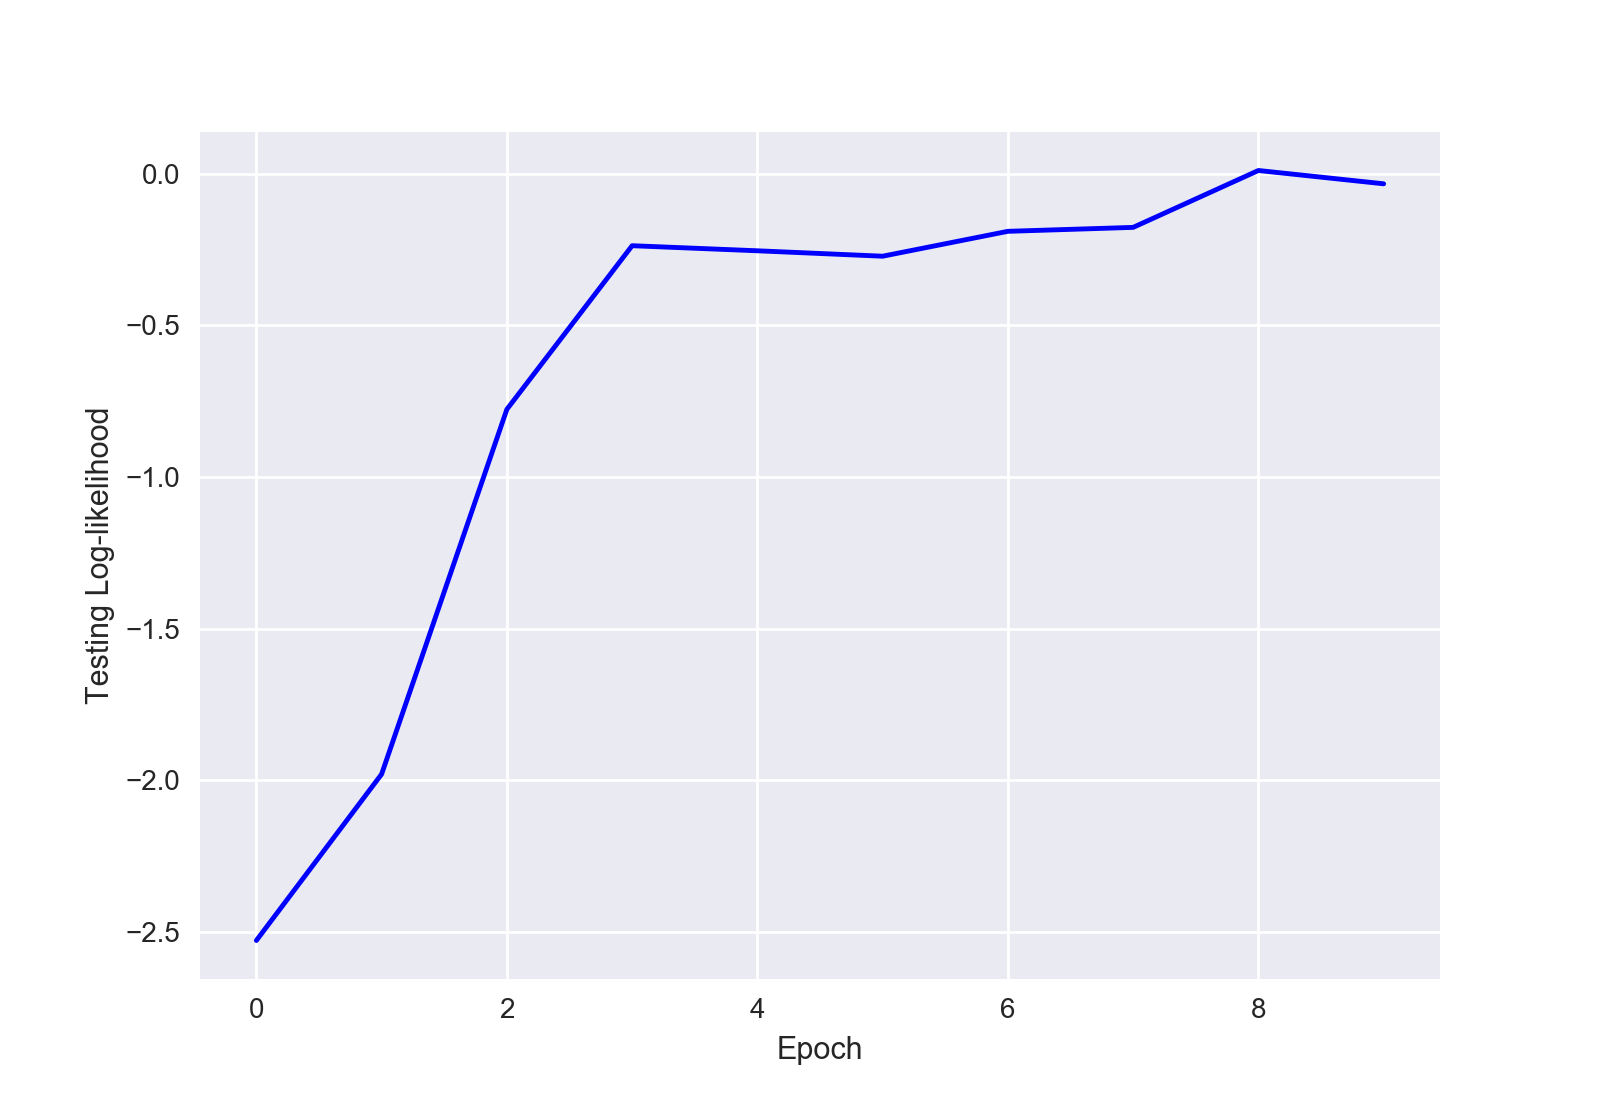
\includegraphics[width=.3\textwidth]{8-2}
	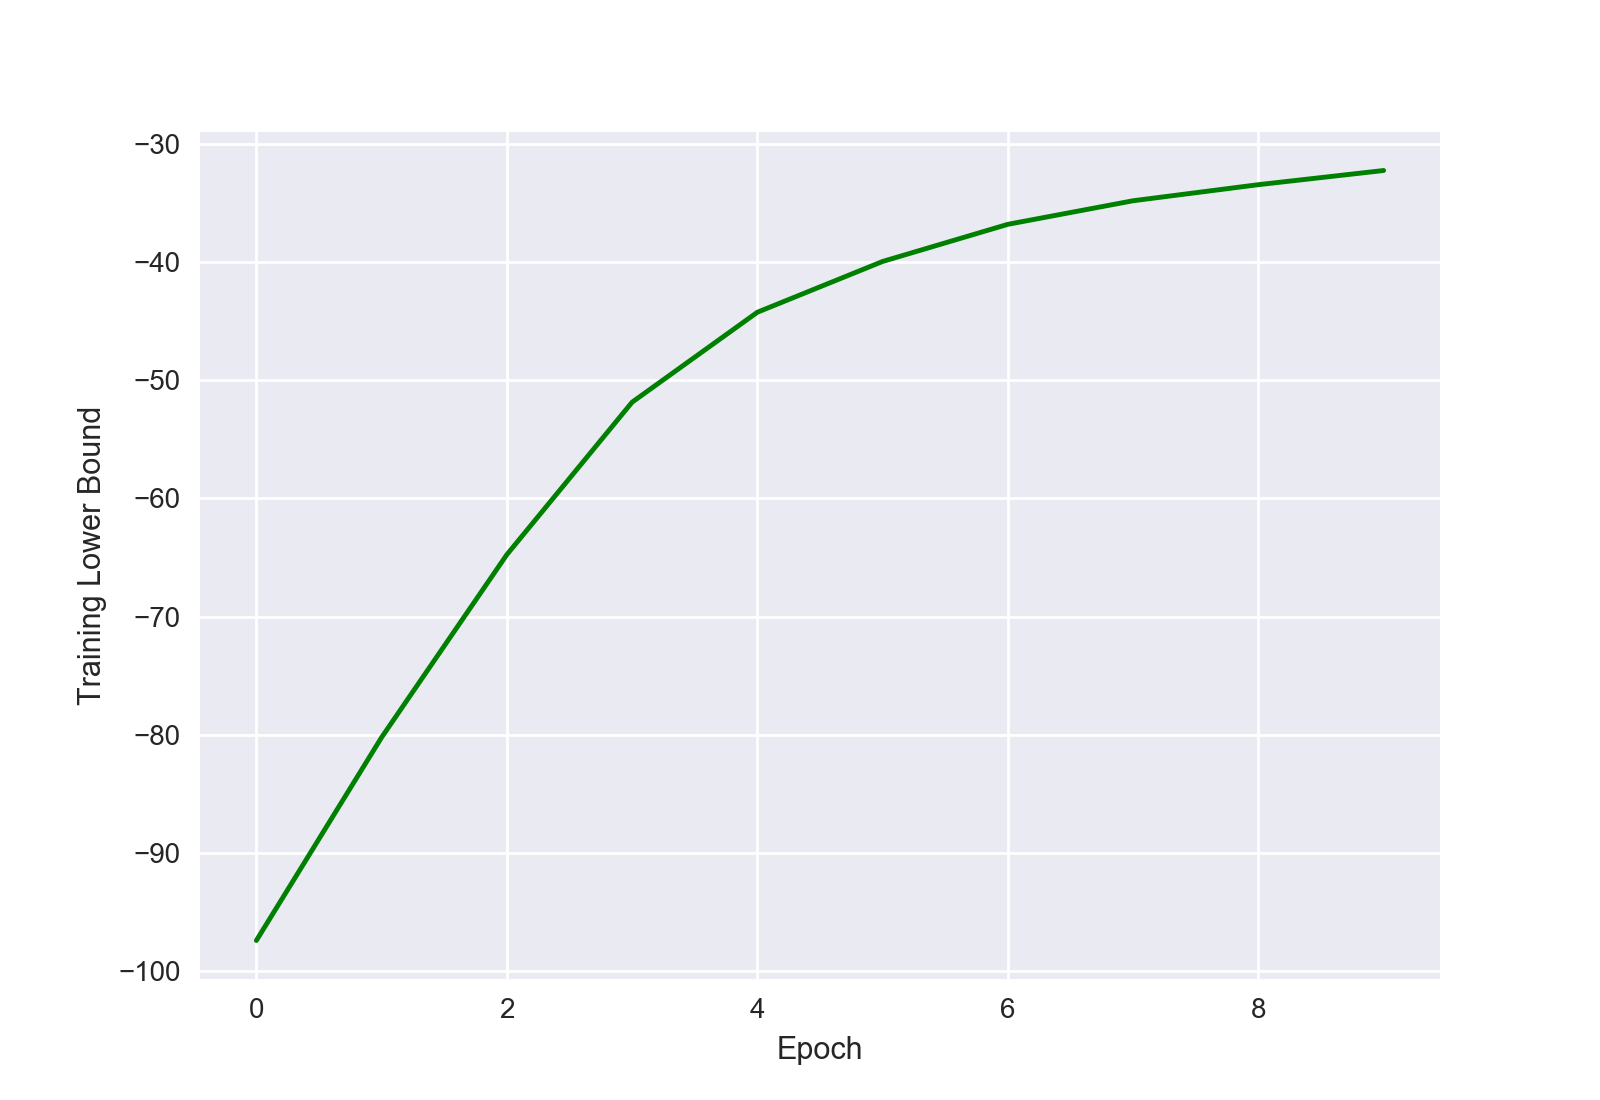
\includegraphics[width=.3\textwidth]{8-3}
	\caption{$K = 8$. Training log-likelihood, testing log-likelihood, and training lower bound for 10 epochs.}
	\label{5}
	\end{figure}

	\begin{figure}
	\centering
	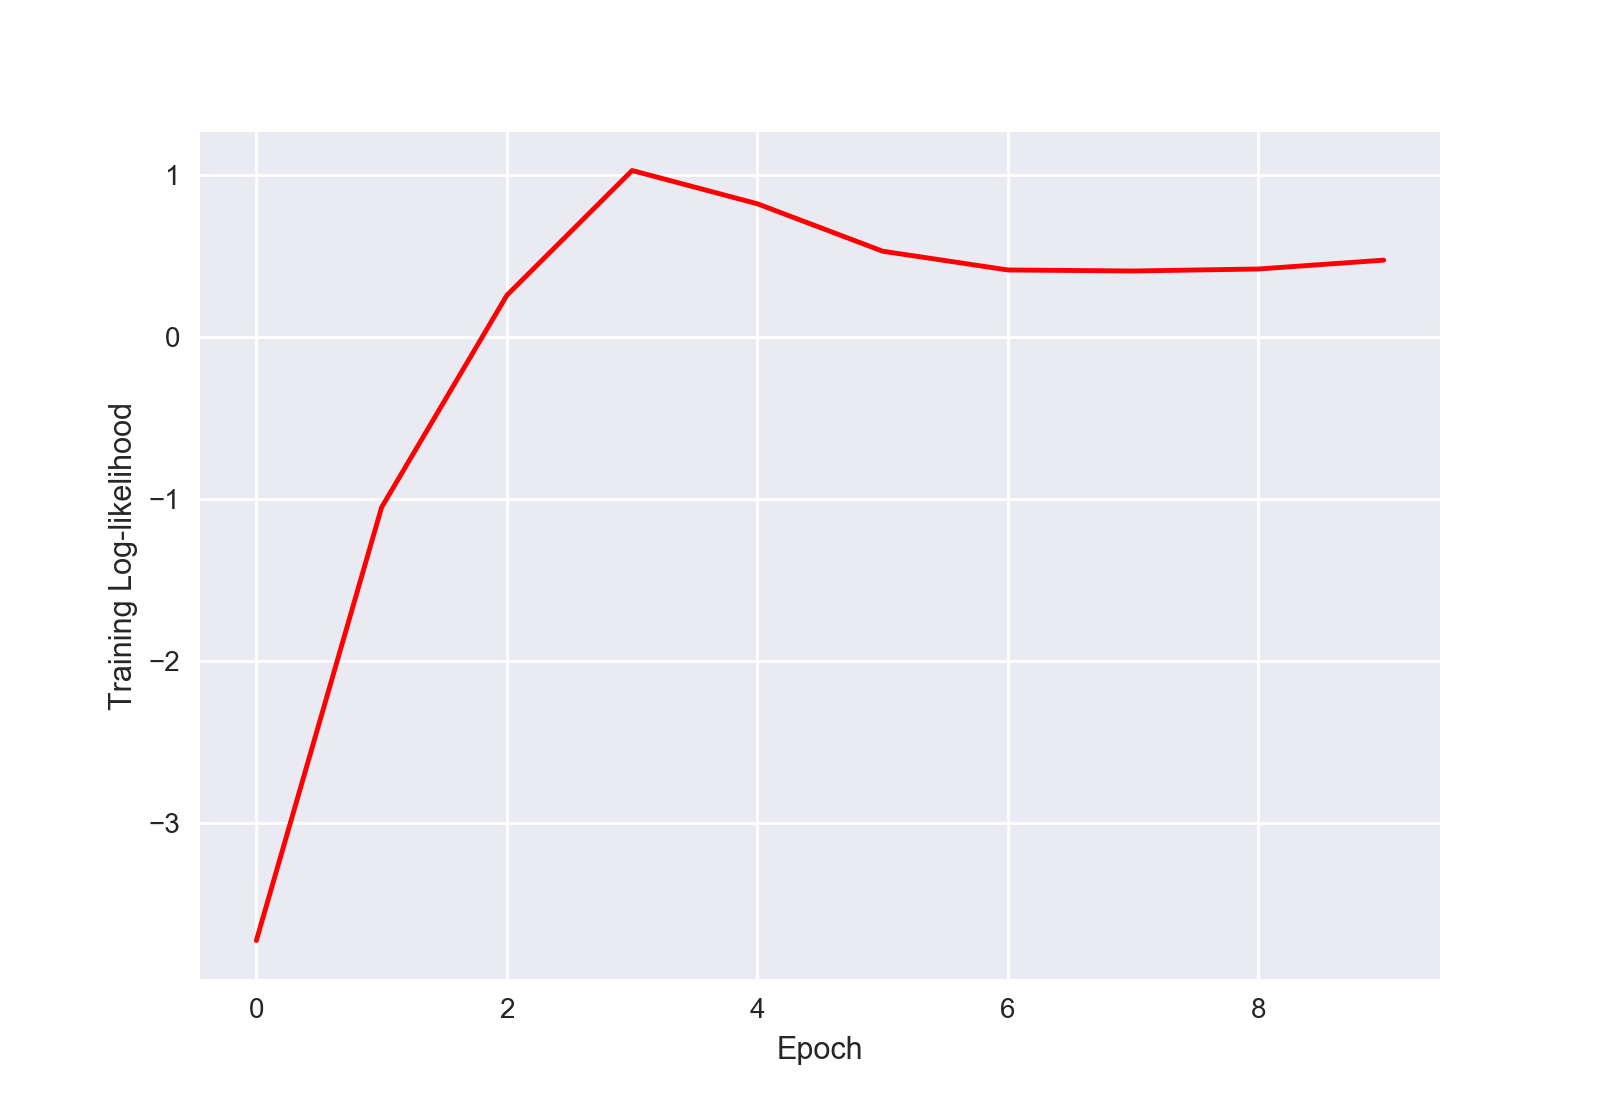
\includegraphics[width=.3\textwidth]{10-1}
	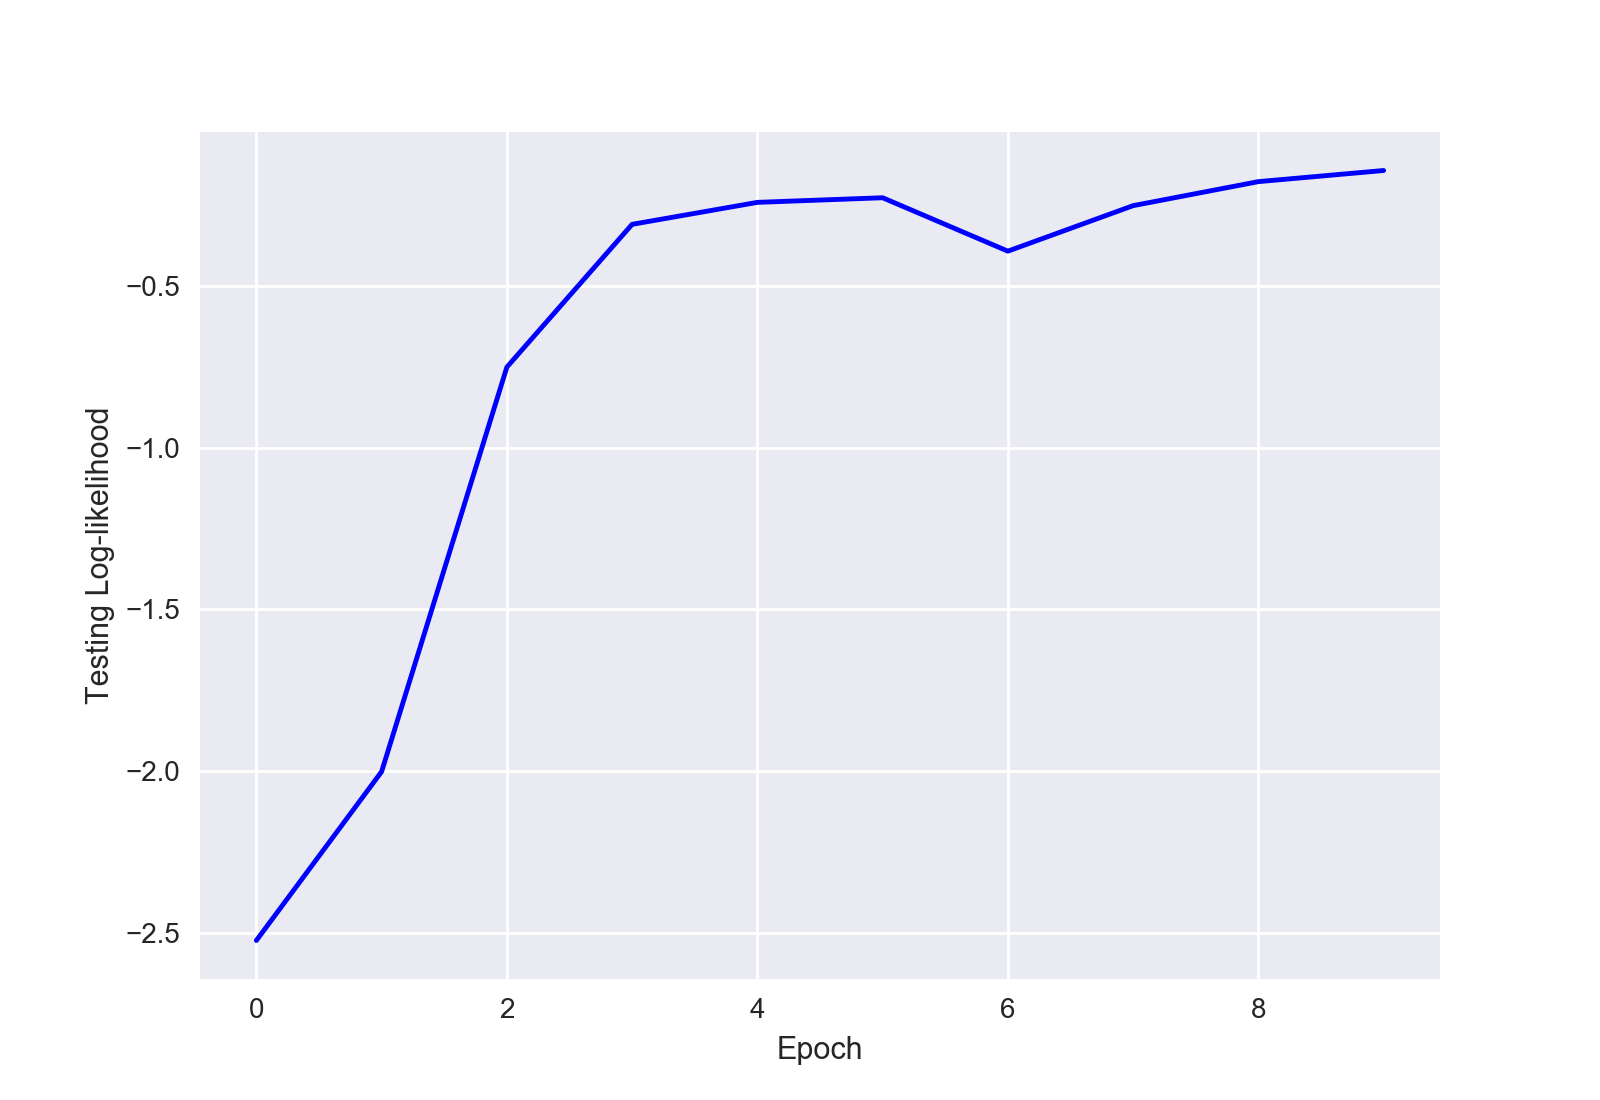
\includegraphics[width=.3\textwidth]{10-2}
	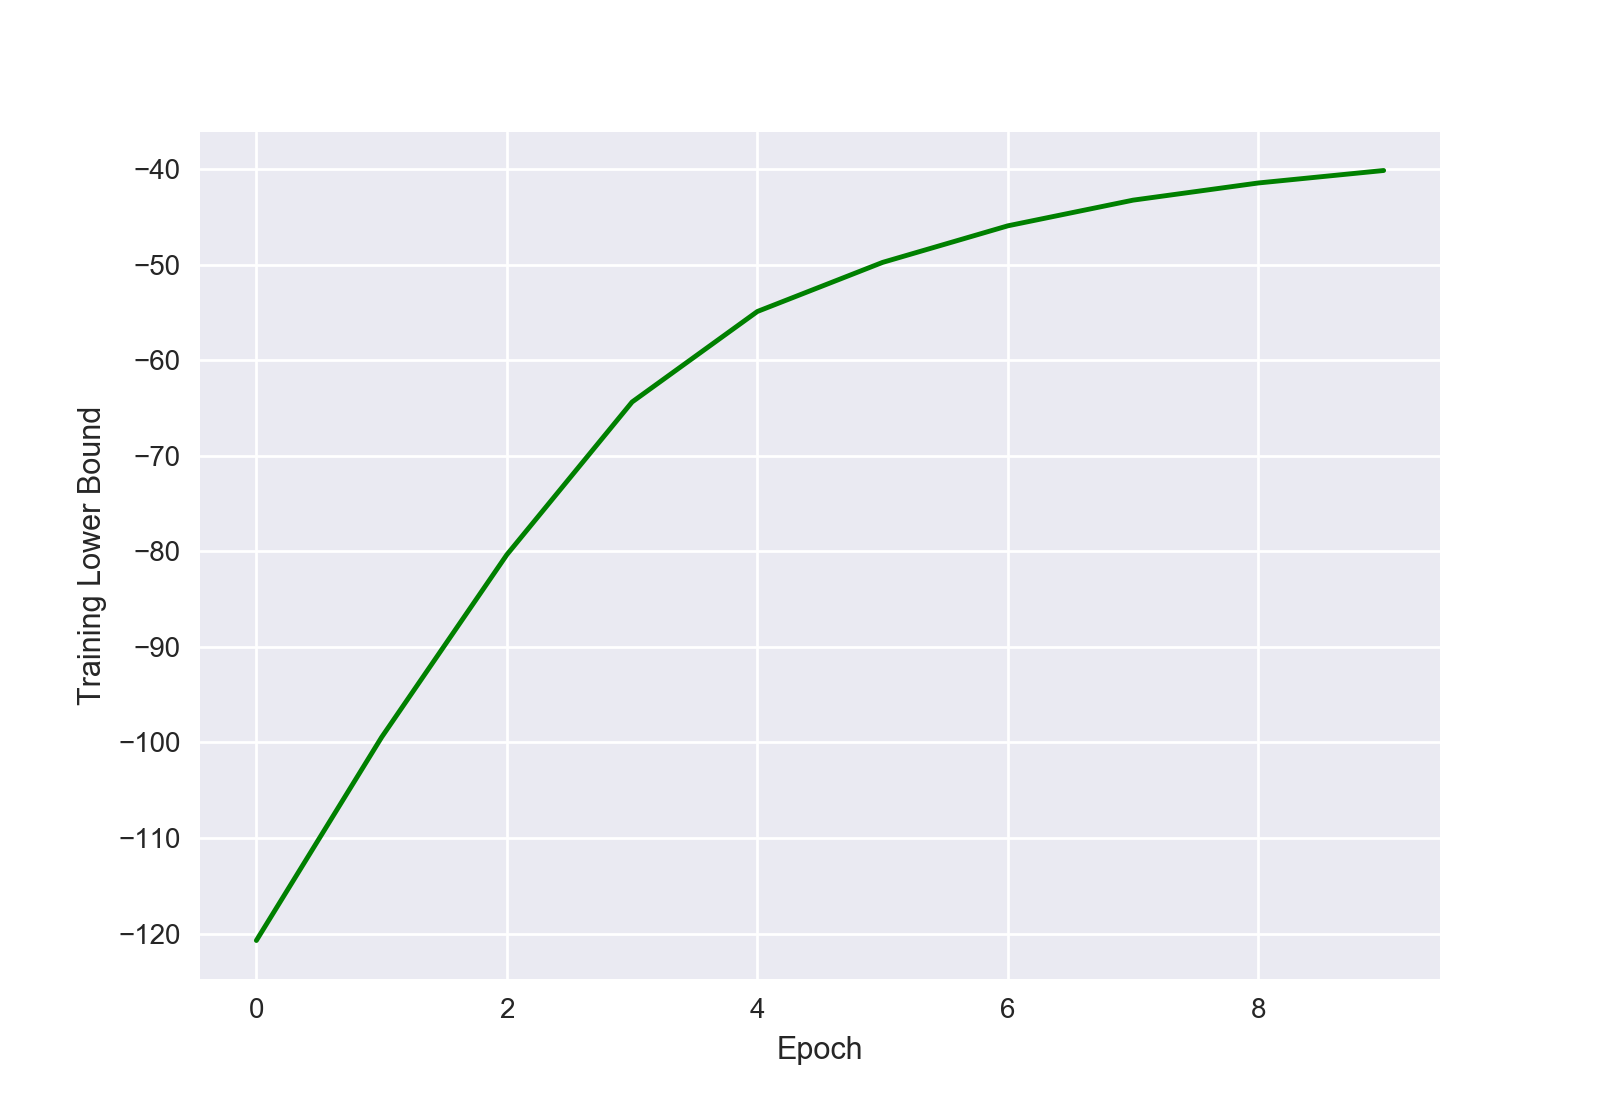
\includegraphics[width=.3\textwidth]{10-3}
	\caption{$K = 10$. Training log-likelihood, testing log-likelihood, and training lower bound for 10 epochs.}
	\label{6}
	\end{figure}


\end{enumerate}

\newpage
\begin{problem}[Gibbs Sampling, 25pts].

  In this problem we will consider a different sampling-based approach for
  estimating the posterior.


\begin{enumerate}

\item Write down the conditional equations for U and V.  That is to say, write their conditional distributions, conditioned on all the other variables as well as the training data:
%
$$p(U_i \ |\ V, R )$$
$$p(V_j \ |\ U, R )$$

Because the model is bi-linear, these updates should have fairly simple forms. Here, we mean $U_i$ to mean the latent parameters corresponding to the $i$th user, and $V_j$ to mean those for the $j$th joke.

\item A Gibbs sampler is an alternative model for computing the posteriors of intractable models.
The method works by repeatedly alternating between drawing samples of $U$ conditioned on $V$, and
then samples of $V$ conditioned on $U$. (We will derive in greater detail in coming classes).

Give the pseudocode for running this algorithm using the posterior equations from above.

\item Run the Gibbs sampler for 100 steps (i.e. update both $U$ and $V$ 100 times).
Plot the training and test-set log-likelihood as a function of the number of steps through your training set.
That is, use all previous samples of $U, V$ to evaluate the predictive probability of all ratings.

\item One reason to be Bayesian is that you don't have to worry about overfitting.
Run your Gibbs sampler for $K = 1$ to $K = 10$, and plot the training and test-set log-likelihood for each value of $K$.  
How do the shapes of these curves differ from the curves you saw when doing maximum likelihood estimation in HW3?


\end{enumerate}
\end{problem}
\begin{enumerate}
	\item Let $J(i)$ be the set of jokes for which user $i$ has supplied a rating. We have
	\begin{align*}
	p(U_i\given V, R) &\propto p(R_i\given U_i, V_{J(i)}) p(U_i) \\
	&= \prod_{j\in J(i)} p(r_{ij}\given U_i, V_j) \prod_{k=1}^K p(u_{ik}) \\
	&= \prod_{j\in J(i)} \mathcal{N}(r_{ij}\given u_i^\top v_j, 1) \prod_{k=1}^K \mathcal{N}(u_{ik} \given 0, 5) \\
	&= \exp\left(-\frac{1}{2} \sum_{j\in J(i)} (r_{ij} - u_i^\top v_j)^2 - \frac{1}{10} u_{i}^\top u_i\right) \\
	&= \exp\left(-\frac{1}{2} \sum_{j\in J(i)} (u_i - \frac{r_{ij}}{v_j^\top v_j}v_j )^\top v_j v_j^\top (u_i - \frac{r_{ij}}{v_j^\top v_j}v_j ) - \frac{1}{10} u_{i}^\top u_i\right) \\
	&= \N(\mu_{iU}, \sigma_{iU}^2),
	\end{align*}
	where 
	\[\mu_{iU} = \sigma_i^2 \sum_{j\in J(i)} (v_j v_j^\top)^{-1} \frac{r_{ij}}{v_j^\top v_j} v_j\]
	\[\sigma_{iU}^2 = \frac{1}{5} I_K + \sum_{j\in J(i)}(v_j v_j^\top)^{-1}\]
	
	Similarly, we have the following conditional for $V$:
	\begin{align*}
	p(V_j\given U, R) &\propto p(R_{:, j}\given U_{I(j)}, V_j) p(V_j) \\
	&= \exp\left(-\frac{1}{2} \sum_{i\in I(j)} (r_{ij} - u_i^\top v_j)^2 - \frac{1}{10} v_{j}^\top v_j\right) \\
	&= \N(\mu_{jV}, \sigma_{jV}^2),
	\end{align*}
	where 
	\[\mu_{jV} = \sigma_j^2 \sum_{i\in I(j)} (u_i u_i^\top)^{-1} \frac{r_{ij}}{u_i^\top u_i} u_i\]
	\[\sigma_{jV}^2 = \frac{1}{5} I_K + \sum_{i\in I(j)}(u_i u_i^\top)^{-1}\]
	
	
	\item Initialize the values of $U_i$ and $V_j$. While not converged, for each variable whose posterior we wish to infer, we sample the value of that variable according to its conditional posterior distribution, given the most recent values of all other variables. In this problem, we would sample the variables $\{U_1,\dots,U_N,V_1,\dots,V_J\}$ in that order every epoch.
	
\end{enumerate}

\end{document}
